
\documentclass[11pt]{article}
\usepackage[utf8]{inputenc}

% Sets page size and margins
\usepackage[letterpaper,top=3cm,bottom=3cm,left=3cm,right=3cm,marginparwidth=2cm]{geometry}
\usepackage{setspace}

% Code in Latex
\usepackage[cache=false]{minted}
\setminted[python]{frame=single, framesep=3mm}

%% Useful packages
\usepackage[justification=centering]{caption}
\usepackage[font=scriptsize,labelfont=bf]{caption}
\usepackage{amsmath}
\usepackage{amssymb}
\usepackage{graphicx}
\usepackage[colorlinks=true, allcolors=black]{hyperref}
\newcommand{\changeurlcolor}[1]{\hypersetup{urlcolor=#1}} 
\usepackage{mathtools}
\usepackage{commath}
\usepackage[protrusion=true,expansion=true]{microtype}

\renewcommand{\vec}[1]{\mathbf{#1}}
\let\oldnorm\norm   % <-- Store original \norm as \oldnorm
\let\norm\undefined % <-- "Undefine" \norm
\DeclarePairedDelimiter\norm{\lVert}{\rVert}

% ---------------------------------------------------------------
% Do Not Change
% ---------------------------------------------------------------
\newcommand{\HRule}[1]{\rule{\linewidth}{#1}} 	% Horizontal rule
\makeatletter							% Title
\def\printtitle{%						
    {\centering \@title\par}}
\makeatother									

\makeatletter							% Author
\def\printauthor{%					
    {\centering \large \@author}}				
\makeatother
% ---------------------------------------------------------------

\title{	\normalsize \textsc{In The Working} 	% Subtitle
		 	\\[2.0cm]								% 2cm spacing
			\HRule{1pt} \\						% Upper rule
			\LARGE \textbf{\uppercase{Machine Learning Overview}}	% Title
			\HRule{2pt} \\ [0.5cm]		% Lower rule + 0.5cm spacing
			\normalsize \today			% Todays date
		}

\author{
		Nicholas Kim\\	
		University College London\\	
		MSc Computational Finance \\ 
}

\begin{document}

\thispagestyle{empty}

\printtitle
        \vfill
\printauthor
\newpage

\setcounter{page}{1}
\section*{About}

This will serve as a short guide to the many functions that can be found in Python's
Scikit-Learn, TensorFlow and Keras libraries. I have created this document to hopefully 
help others learn more about the area of Machine Learning and its capabilities. As a Note
this paper, will not serve as a comprehensive guide to Machine Learning but more as a 
cheat sheet to help one remember certain functions that are contained in the libraries 
mentioned above. \\

\noindent 
This guide will continually be updated as libraries are changed and/or new 
functions are added. I have also not gone through these libraries in full and will add 
in what I have been able to cover so far. \\ 

\noindent 
Please feel free to reach out to me at 
\href{mailto:Nicholaskim46@gmail.com}{Nicholaskim46@gmail.com} if there are any typos or
mistakes throughout this guide.

\pagebreak

\tableofcontents

\pagebreak

\section{Training Models/Algorithms}

\subsection{Linear Regression}

\textit{Linear Regression} simply makes a prediction by computing a weighted sum of the input
features, plus a constant term which is called the bias (Intercept)

$$\hat{y} = \theta_{0} + \theta_{1}x_{1} \cdots + \theta_{n}x_{n}$$

\noindent 
In the equation above:
\begin{itemize}
    \item $\hat{y}$, is the predicted value
    \item $n$, is the number of features
    \item $x_{i}$, is the $i^{th}$ feature values
    \item $\theta_{j}$ is the $j^{th}$ model parameter (including the bias term $\theta_{0}$
    and the feature weights $\theta_{1}, \theta_{2}, \cdots, \theta_{n}$)
\end{itemize}

\noindent 
However, this equation can be written much more concisely using a vectorized form:

$$\hat{y} = \vec{h_{\theta}(x)} = \vec{\theta \cdot x}$$

\noindent 
Where we have the following:
\begin{itemize}
    \item $\vec{\theta}$, is the model's \textit{parameter vector}, conatining the bias term
          $\theta_{0}$ and the feature weights $\theta_{1}$ to $\theta_{n}$.
    \item $\vec{x}$, is the instance's \textit{feature vector}, containing $x_{0}$ to $x_{n}$
          with $x_{0}$ always eqaul to 1.
    \item $h_{\theta}$, is the hypothesis function, using the model parameters $\vec{\theta}$
\end{itemize}

\noindent
Now for training the model we want to minimize the Mean Squared Error (MSE). This
means that we need to find a value for $\vec{\theta}$ such that it minimizes the MSE. It is 
also very common to see Root Mean Squared Error (RMSE) as a performance measure of a regression
model. \\

\noindent 
The MSE of a Linear Regression is shown below:

$$\text{MSE}(\vec{X}, h_{\theta}) = \frac{1}{m} \sum^{m}_{i = 1} (\vec{\theta}^{\intercal}\vec{x^{(i)}} - y^{(i)})^{2}$$

\subsection{Gradient Descent}

\textit{Gradient Descent} is a optimization algorithm capable of finding optimal 
solutions to a wide range of problems. The general idea of this algorithm is to tweak parameters
iteratively in order to minimize a cost function.\\

\noindent 
An intuitive way to think about Gradient Descent is imagine one is trying to find
the fastest way to reach a bottom of a valley. A good strategy would be to go downhill in 
the direction of the steepest slope. This is exactly what Gradient Descent does: it measures
the local gradient of the error function with regard to the parameter vector $\vec{\theta}$,
and it goes in the direction of the descending gradient. \\

\noindent
To implement \textit{Gradient Descent}, we need to compute the gradient of the cost function with
regard to each model parameter $\theta_{j}$. Thus, we need to take the partial derivative of the 
cost function with respect to each $\theta_{j}$. This can be seen below:

$$\frac{\partial}{\partial \theta_{j}} \text{MSE}(\vec{\theta}) = \frac{2}{m} \sum^{m}_{i = 1} (\vec{\theta}^{\intercal} \vec{x}^{(i)} - y^{(i)}) x_{j}^{(i)}$$

\noindent
Additionally, instead of computing partial derivatives individually, we can also use the following
equation to compute the gradient vector for MSE.

$$
\nabla_{\theta} \text{MSE}(\vec{\theta}) =  
\begin{pmatrix}
\frac{\partial}{\partial \theta_{0}} \text{MSE}(\vec{\theta}) \\ \\
\frac{\partial}{\partial \theta_{1}} \text{MSE}(\vec{\theta}) \\ 
\vdots \\ 
\frac{\partial}{\partial \theta_{n}} \text{MSE}(\vec{\theta})
\end{pmatrix}
= \frac{2}{m}\vec{X}^{\intercal}(\vec{X}\theta - \vec{y})
$$ \\

\noindent
Once we have the gradient vector, which points uphill, we just go in the opposite direction. This means
that we need to subtract the $\nabla_{\theta}\text{MSE}(\theta)$ from $\theta$. Here we will use 
$\eta$ as our learning rate parameter for each step. We will multiply the gradient vector by $\eta$ to 
determine the size of the downhill step.

$$\vec{\theta}^{(\text{next step})} = \theta - \eta \nabla_{\theta} \text{MSE}(\theta)$$ 

\noindent
From the equation above we can see how important $\eta$ is, when training optimizing training for 
gradient descent. 

\noindent
Below will be important notes for Gradient Descent:

\begin{itemize}
    \item $\mathbf{\theta}$, this vector is initialized with random values
    (\textit{Random Initialization}), and it is then improved gradually, taking one step at a
    time to decrease the cost function.

    \item \textbf{Learning Rate}, $\eta$, this parameter determines how large the "learning" will be in each
    iteration of the algorithm. If the learning rate is too small then it will take too
    long to converge to the desired state, and on the other hand, if it is too large then
    the algorithm will never be able to converge as it will be bouncing around the cost
    function. It is important to note that it is often optimal to set the learning rate dynamically so that
    initially we have a high learning rate to get faster convergence to the optimal, and then slowly decrease
    the learning rate as we get closer to the optimal point.

    \item Finally, not all cost functions are bowl shaped. This means we can have cost functions
    that have holes, ridges, plateaus, and all other forms of irregular terrain, making convergence
    of this alorgithm difficult. However, this can be helped by the optimization of the learning rate.
\end{itemize}

\subsection{Polynomial Regression}

\textit{Polynomial Regression}, can be done by adding powers to each feature, then training a linear
on this set of extended features. Using Scikit-Learn's \mintinline{python}{PolynomialFeatures} class, we can
transform our training data using the following code: \\

\begin{minted}{python}
from sklearn.preprocessing import PolynomialFeatures
from sklearn.linear_model import LinearRegression

m = 100
X = 6 * np.random.rand(m, 1)
y = 0.5 * X**2 + X + 2 + np.random.randn(m, 1)

poly_features = PolynomialFeatures(degree=2, include_bias=False)
X_poly = poly_features.fit_transform(X)

lin_reg = LinearRegression()
lin_reg.fit(X_poly, y)
\end{minted} 

\noindent
\\ Now \mintinline{python}{X} is transformed into \mintinline{python}{X_poly} where it now contains the original features of \textbf{X}
plus the squares of this feature (Also note that as we increase variables, this fuction will also include all
the cross terms. For example, if we have variables \textit{a} and \textit{b} with degree=3, we add the features
$a^{2}, a^{3}, b^{2}, b^{3}, ab, a^{2}b, ab^{2}$). We then fit the new features \mintinline{python}{X_poly} 
with Scikit-Learns's \mintinline{python}{LinearRegression}, which returns us a quadratic polynomial regression. \\

\noindent
\textbf{Warning}: \textit{PolynomialFeatures(degree=d)} transforms an array continaing \textit{n} features into
an array containing $\frac{(n+d)!}{d!n!}$ features. So we must take care in the explosion of the number of 
features.

\subsection*{Bias/Variance Trade Off}

\begin{itemize}
    \item \textbf{Bias}
        \begin{itemize}
            \item This part of the generalization error is due to wrong assumptions, 
            such as assuming that the data is linear when it is actually quadratic. A 
            high-bias model is most likely to underfit the training data.
        \end{itemize}
    \item \textbf{Variance}
        \begin{itemize}
            \item This part is due to the models excessive sensitivity to small variations
                  training data. A model with many degrees of freedom (such as high-degree)
                  polynomial model) is likely to have high variance and thus overfit the 
                  training data.         
        \end{itemize}
    \item \textbf{Irreducible Error}
        \begin{itemize}
            \item This is due to the noisiness of data itself. The only way to reduce this
                  part of the error is to clean up the data (e.g., fix the data sources,
                  such as broken sensors, or detect and remove outliers)
        \end{itemize}
    \item Generally, increasing a model complexity till typically increase its variance
          and reduce its bias. Conversely, reducing a model's complexity increases its bias
          and reduces its variance. This is the reason for this so-called trade off
    \item The optimal strategy would be to find the intersection that minimizes both the 
          bias and variance.
\end{itemize}

\subsection{Regularized Linear Models}

Regularizing linear models is a great way to reduce the chance of overfitting the data that
it is using to be trained. This is the case as it helps reduce the amount of degrees of 
freedom that the model has. \\

\noindent 
In this section we will take a look at three different regularized linear models: 
Ridge Regression, LASSO, Elastic Net.

\subsubsection{Ridge Regression}

\textit{Ridge Regression}, is a regualrized linear regression with a regularization term
eqaul to:  $\alpha \sum_{i=1}^{n} \theta_{i}^{2}$, which is then added to the cost function.
This forces the algorithm to not only fit the data but to keep the models weights as small
as possible. \\

\noindent 
It is important to note that we want to keep the regularization term during
\textbf{training only} and once deployed, the regularization term should be dropped.\\

\noindent 
The hyperparameter $\alpha$ controls how much we want to regularize the model.
If $\alpha = 0$ then the model is just a linear regression, however, if $\alpha$ is very
large, then all the weights end up very close to zero. Where the result will be a flat line
going through the data's mean.\\

\noindent 
Below will be the total cost function for Ridge Regression:

$$J(\theta) = \text{MSE}(\theta) + \alpha \frac{1}{2} \sum_{i=1}^{n} \theta_{i}^{2}$$

\noindent 
Note that the biased term $\theta_{0}$ is not regularized (the sum starts at $i=1$, 
not 0). If we define $\vec{w}$ as the vector of feature weights 
($\theta_{1} \text{ to } \theta_{n}$), then the regularization term is equal to 
$\frac{1}{2}(\norm{\vec{w}}_{2})^{2}$ represents the $l_{2}$ norm of the weight vector. \\ 

\subsubsection*{Intuitive Explanation of $l_{2}$ norm}
\noindent 
The $l_{2}$ norm penalizes the square of the weights in the model. Therefore, it is much
more inclined to push down the big weights as compared to the smaller weights. This is the reason why
we see weights get pushed down close to zero for this model but never all the way to zero. \\

\noindent 
\textbf{Remember}, it is important to scale the data 
(e.g., using \textit{StandardScaler} in Pythons Scikit-Learn) before performing Ridge Regression,
as the model is sensitive to the scale of input features. This holds for most regularized models.

\subsubsection{LASSO}

\textit{Lease Absolute Shrinkage and Selection Operator Regression (LASSO)} is another version
of a regularized version of Linear Regression: just like Ridge Regression, it adds a
regularization term to the cost function, but it uses a $l_{1}$ norm of the weight vector
instead of half the square of the $l_{2}$ norm. \\

\noindent
Below will be the LASSO Regression Cost Function:

$$J(\vec{\theta}) = \text{MSE}(\vec{\theta}) + \alpha \sum_{i = 1}^{n} \abs{\theta_{i}}$$

\noindent 
A very important characteristic of Lasso Regression is that it tends to eliminate the 
weights of the least important features (i.e., set them to zero). In other words, Lasso Regression
automatically performs feature selection and outputs a \textit{sparse model} (i.e., with few
nonzero weights).\\

\subsubsection*{Intuitive Explanation of $l_{1}$ norm}
\noindent 
LASSO tends to send coefficients to zero because it tries to minimize the absolute value
of the weights, thus it is inclined to make big weights smaller and small weights smaller as well. 
Therefore, it tends to drive the weights to 0, which then brings upon a sparse weight vector.

\subsubsection{Elastic Net}

\textit{Elastic Net} is the middle ground between Ridge Regression and Lasso Regression. The 
regularization term is a simple mix of both Ridge and Lasso's regularization terms, and this can be 
controlled with the mix ratio $r$. When $r = 0$, Elastic Net is equal to Ridge Regression, and when
$r = 1$, it is equivalent to Lasso Regression. \\

\noindent 
Below will be the cost function for Elastic Net:

$$J(\vec{\theta}) = \text{MSE}(\vec{\theta}) + r\alpha \sum_{i=1}^{n} \abs{\theta_{i}} + \frac{1-r}{2} \alpha \sum_{i=1}^{n} \theta_{i}^{2}$$

\subsubsection{When to use Linear Regression, LASSO, Ridge, or Elastic Net?}

It is almost always perferable to have at least a little bit of regularization, so generally,
plain Linear Regression should be avoided. Ridge Regression, is usually a good default for solving
linear problems, however, if we suspect that there may be only a few features that are useful, we 
should prefer to use Lasso or Elastic Net. As discussed earlier, it is preferred to use Lasso or 
Elastic Net when we want to try and reduce the least important features in a dataset to zero. \\

\noindent 
In general, Elastic Net is preferred over Lasso as sometimes the model can behave 
erratically when the number of features is greater than the number of training instances or when
several features are strongly correlated. 

\subsection{Logistic Regression}

\textit{Logistic Regression} (Also called \textit{Logit Regression}) is a regression that is
commonly used to estimate the probability that an instance belongs to a particular class. If the 
probability is greater than 50\%, then the model predicts that the instance belongs to that class
and otherwise it does not. This trait makes it a \textit{binary classifier}.

\subsubsection{Estimating Probabilities}

Logistic Regression works just like a Linear Regression model, it computes a weighted sum of the
input features (plus a bias term), but instead of outputting the result directly like the Linear
Regression model, it outputs the \textit{logistic} of this result (See Below).

$$\hat{p} = h_{\theta}(\vec{x}) = \sigma(\vec{x}^{\intercal}\vec{\theta})$$

\noindent 
The logistic -- noted $\sigma(\cdot)$ -- is a \textit{sigmoid function} (i.e., S-Shaped)
that outputs a number between 0 and 1. It is defined below:

$$\sigma(t) = \frac{1}{1 + \text{exp}(-t)}$$

\noindent 
Once the Logistic Regression model is able to estimate the probability $\hat{p} = h_{\theta}(\vec{x})$
that an instance $\vec{x}$ belongs to the positive class, it can make the prediction for $\hat{y}$
easily using the function below:

\[ \hat{y} = 
\begin{cases} 
    0 & \text{if } \hat{p} < 0.5 \\
    1 & \text{if } \hat{p} \geq  0.5 
\end{cases}
\] \\

\noindent 
\textbf{Note}: The score $t$ is often called the \textit{logit}. This comes from the 
fact that the logit function is defined as $\text{logit}(p) = \text{log}(\frac{p}{1-p})$, this is
the inverse of the logistic function. The logit is also called the \textit{log-odds}, since it is
the log of the ratio between the estimated probability for the positive class and the estimated
probability for the negative class.

\subsubsection{Training and Cost Function}

The objective of training a Logistic Regression is to set the parameter vector $\vec{\theta}$ so 
that the model estimates high probabilities for positive instances ($y = 1$) and low probabilities
for negative instances ($y = 0$). This idea is captured by the cost function shown below for a 
single training instance $\vec{x}$:

\[ c(\vec{\theta}) = 
\begin{cases} 
    \text{-log}(\hat{p}) & \text{if } y = 1 \\
    \text{-log}(1 - \hat{p}) & \text{if } y = 0
\end{cases}
\] \\

\noindent 
Intuitively, we can see the cost function makes sense. As $t$ approaches 0 we can see that 
$-\text{log}(t)$ grows very large, so the cost will be large if the model estimates a probability
close to 0 for a positive instance, and it will also be very large if the model estimates a 
probability close to 1 for a negative instance. On the other hand, we can see that the cost will
be very small is the model is able to estimate the instance correctly. \\

\noindent 
The cost function over the whole training set is the average cost over all training 
instances. It can be shown in a single expression called the \textit{log loss}, shown below:

$$J(\vec{\theta}) = -\frac{1}{m} \sum_{i=1}^{m} [y^{(i)} \text{log}(\hat{p}^{(i)}) + (1-y^{(i)})\text{log}(1-\hat{p}^{(i)})]$$

\noindent 
There is no closed-form equation to compute the value of $\vec{\theta}$ that minimizes this
cost function. However, this cost function is convex, so Gradient Descent (or other optimization
algorithms) is guaranteed to find the global minimum.\\

\noindent 
The partial derivatives of the cost function w.r.t. the $j^{th}$ model parameter $\theta_{j}$
is shown below:

$$\frac{\partial}{\partial \theta_{j}} J(\vec{\theta}) = \frac{1}{m} \sum_{i=1}^{m} (\sigma(\vec{\theta}^{\intercal}\vec{x}^{(i)})-y^{(i)})\vec{x}_{j}^{(i)}$$

\noindent 
For each instance, it computes the prediction error and multiplies it by the $j^{th}$
feature value, and then it computes the average over all training instances. Once we are able to get
the gradient vector containing all the partial derivatives, we can use it in Batch Gradient Descent
algorithm (So on with Stochastic Gradient Descent and Mini-batch Gradient Descent).



\section{Classification}

In this section, we will be covering the basics of classification machine learning techniques. Topics
will range from what data to use for learning, how to train a Multiclass/binary classifiers, 
look over different performance measures and finally looking over multioutput classifiers. 

\subsection{MNIST}

In this section we will be utilizing the MNIST dataset, which is made up of 70,000 images of digits
written by hand. Each image is labeled with the digit it is an image of. This is one of the most 
popular datasets for intially learning about the world of Machine Learning (Equivalent to the 
"Hello World" program when first learning how to code).\\

\noindent
Fortunately, Scikit-Learn provides a very easy way to obtain this data. Using the following block
of code we can obtain this dataset:

\begin{minted}{python}
from sklearn.datasets import fetch_openml
mnist = fetch_openml("mnist_784", version=1)
mnist.keys()

# Below will be the dictionary for this dataset
'''
dict_keys(['data', 'target', 'feature_names', 'DESCR', 'details',
           'categories', 'url'])
'''
\end{minted}

\noindent
Datasets from Scikit-Learn have mostly the same dictionary structure:

\begin{itemize}
    \item A \mintinline{python}{DESCR} key describes the dataset
    \item A \mintinline{python}{data} key contains an array with one row per instance and one column
    per feature
    \item A \mintinline{python}{target} key containing an array with all the labels for each respective
    image that is in the data
\end{itemize}

\noindent
Lets take a look at the shape of the dataset:

\begin{minted}{python}
X, y = mnist["data"], mnist["target"]
X.shape # (70000, 784)
y.shape # (70000,)    
\end{minted}

\noindent 
Here we see, as mentioned earlier, that there is 70,000 images with each image containing 784 
features. There are 784 features as each image is 28 x 28 pixels, and each feature represents the pixels
density ranging from 0 (white) to 255 (black). Additionally, we see that the target data is just 
70,000 labels for each respective image in X. \\ 

\noindent
Finally, we should always split the data before inspecting the data more closely. We can make the 
test and training sets in the following manner:

\begin{minted}{python}
X_train, X_test = X[:60000], X[60000:]
y_train, y_test = y[:60000], y[60000:]    
\end{minted}

\noindent
\textbf{Note:} that this dataset has already been shuffled. However, if this dataset has not been
shuffled then it is crucial that we do this before splitting the data as we do not want some folds
when doing cross-validation to be missing digits.

\subsection{Training a Binary Classifier}

For simplification reasons, we will first only try to identify one digit, number 5. This classifier 
will be a \textit{binary classifier}, capable of distinguishing between just 2 classes 5 and not a 5.\\

\noindent
First we will create target vectors for this classification task:

\begin{minted}{python}
y_train_5 = (y_train == 5) # True for all 5s, False for all others
y_test_5 = (y_test == 5)
\end{minted}

For this example we will be using the \textit{Stochastic Gradient Descent} (SGD) classifier, using 
Scikit-Learn's \mintinline{python}{SGDClassifier} class. This classifier is advantageous because it 
is able to handle large datasets efficiently. This is the calse because SGD deals with training instances
independently, one at a time.\\

\noindent
Below will be some code that is implementing this classifier:

\begin{minted}{python}
from sklern.linear_model import SGDClassifier

sgd_clf = SGDClassifier(random_state=42)
sgd_clf.fit(X_train_5, y_test_5)    
\end{minted}

\noindent
Now that the model is trained we, hope, that we can now predict with reasonable accuracy that a 
number is a 5 and not a 5 if it is some other digit.

\subsection{Performance Measures}

Here we find that evaluating a classifier tends to be much trickier than evaluating a regression based
model. In this section, we will be spending a lot of time going over the many different performance
measures there are available. 

\subsubsection{Measuring Accuracy Using Cross-Validation}

A common way to evaluate a model is to just use cross-validation. Here we will be using a off the shelf
cross validation function, but if you need more control over the cross-validation processs then you 
can always build your own. \\

\noindent
Below will be the implementation using Sciki-Learn's \mintinline{python}{cross_val_score()} function
to evaluate our \mintinline{python}{SGDClassifier} we trained earlier. Note, that we are using K-folds
cross-validation when using the python function \mintinline{python}{cross_val_score()}.

\begin{minted}{python}
from sklearn.model_selection import cross_val_score
# Splits training set into 3 folds, then making predictions and 
# evaluating them on each fold using a model trained on the remaining
# folds.
cross_val_score(sgd_clf, X_train, y_train, cv = 3, scoring='accuracy')

# Output:
# array([0.96355, 0.93795, 0.95615])
\end{minted}

\noindent
After cross-validation we see that the model has an accuracy of above 93\% on all cross-validation 
folds. However, there is a catch to this. We will now fit a "very dumb" classifier that just 
classifies every image as a "not-5" class:

\begin{minted}{python}
from sklearn.base import BaseEstimator

class Never5Classifier(BaseEstimator):
    def fit(self, X, y=None):
        pass
    def predict(self, X):
        return np.zeros((len(x), 1), dtype=bool)

never_5_clf = Never5Classifier()
cross_val_score(never_5_clf, X_train, y_train, cv=3, scoring='accuracy')

# Output:
# array([0.91125, 0.90855, 0.90915])
\end{minted}

\noindent
Woah, we have over 90\% accuracy on the dataset by just classifying everything as not a 5. This is 
because we only have about 10\% of the images as 5s, so if we always guess that the image is not a 
5 then we will be right about 90\% of the time. \\

\noindent 
The above is a prime example why accuracy is generally not the preferred performance measure for 
classifiers, especially when we are dealing with \textit{skewed datasets} (i.e., when some classes
are much more frequent then others).

\subsubsection{Confusion Matrix}

Another way to evaluate performance of a classfier is to look at the \textit{Confusion Matrix}. In
general, the idea of this matrix is to count the number of times instances of a class A are classified
as a class B. \\ 

\noindent
To create the confusion matrix, we need to first have a set of predictions so that they can be compared
to the actual targets. As we generally do not want to touch the test set until the model is complete,
we can use \mintinline{python}{cross_val_predict()} instead to generate our predictions against the 
target:

\begin{minted}{python}
from sklearn.model_selection import cross_val_predict()
from sklearn.metrics import confusion_matrix

y_train_pred = cross_val_predict(sgd_clf, X_train, y_train_5, cv=3)

confusion_matrix(y_train_5, y_train_pred)

'''
Output:
Confusion Matrix Below:
array([[53057,  1522],
       [ 1325,  4096]])
'''
\end{minted}

\noindent
Similarly as above, \mintinline{python}{cross_val_predict()}, also performs K-fold cross-validation,
but instead of returning scores, it returns the predictions made on each test fold. Now for the
confusion matrix:\\

\noindent 
\textbf{Confusion Matrix Explanation}
\begin{itemize}
    \item Each \textbf{Row} in a confusion matrix represents an \textit{actual class}
    \item Each \textbf{Column} in a confusion matrix represents a \textit{predicted class}
\end{itemize}

\noindent
In the case for this model, the \textbf{first row} of the matrix above considers non-5 images (negative class):
53,057 of them were correctly classified as non-5s (called \textit{True Negatives}), while the 
remaining 1,522 were wrongly classified as 5s (\textit{False Positives}). The \textbf{second row}, 
considers the images of 5s (\textit{positive class}): 1,325 were wrongly classified as non-5s 
(\textit{false negatives}), while the remaining 4,096 were correctly classified as 5s (\textit{True Positives}).
Additionally, a perfect classifier would only have non-zero values on the main diagonal. 

\subsubsection{Precision and Recall}

Although the \textit{confusion matrix} may give a lot of information, sometimes it is better to look at a more 
straight-forward metric. Both \textit{Precision} and \textit{Recall} are great for this task.

\subsubsection*{Precision}

\textit{Precision}, can be defined as the accuracy of the positive prediction for the classifier we are evaluating.
Below will be the formula to calculate precision:

$$\text{Precision} = \frac{\text{TP}}{\text{TP} + \text{FP}}$$

\noindent 
Where:
\begin{itemize}
    \item TP $\rightarrow$ The number of true positives
    \item FP $\rightarrow$ The number of false positives
\end{itemize}

\subsubsection*{Recall}

\textit{Recall}, can be defined as the \textit{sensitivity} or the \textit{true positive rate} (TPR):
this is the ratio of positive instances that are correctly detected by the classifier. The 
equation for Recall can be defined as follows:

$$\text{Recall} = \frac{\text{TP}}{\text{TP} + \text{FN}}$$

\noindent
Where, FN, is the number of false negatives. Additionally, below we can see a more detailed 
version of the confusion matrix to help clear any confusion:

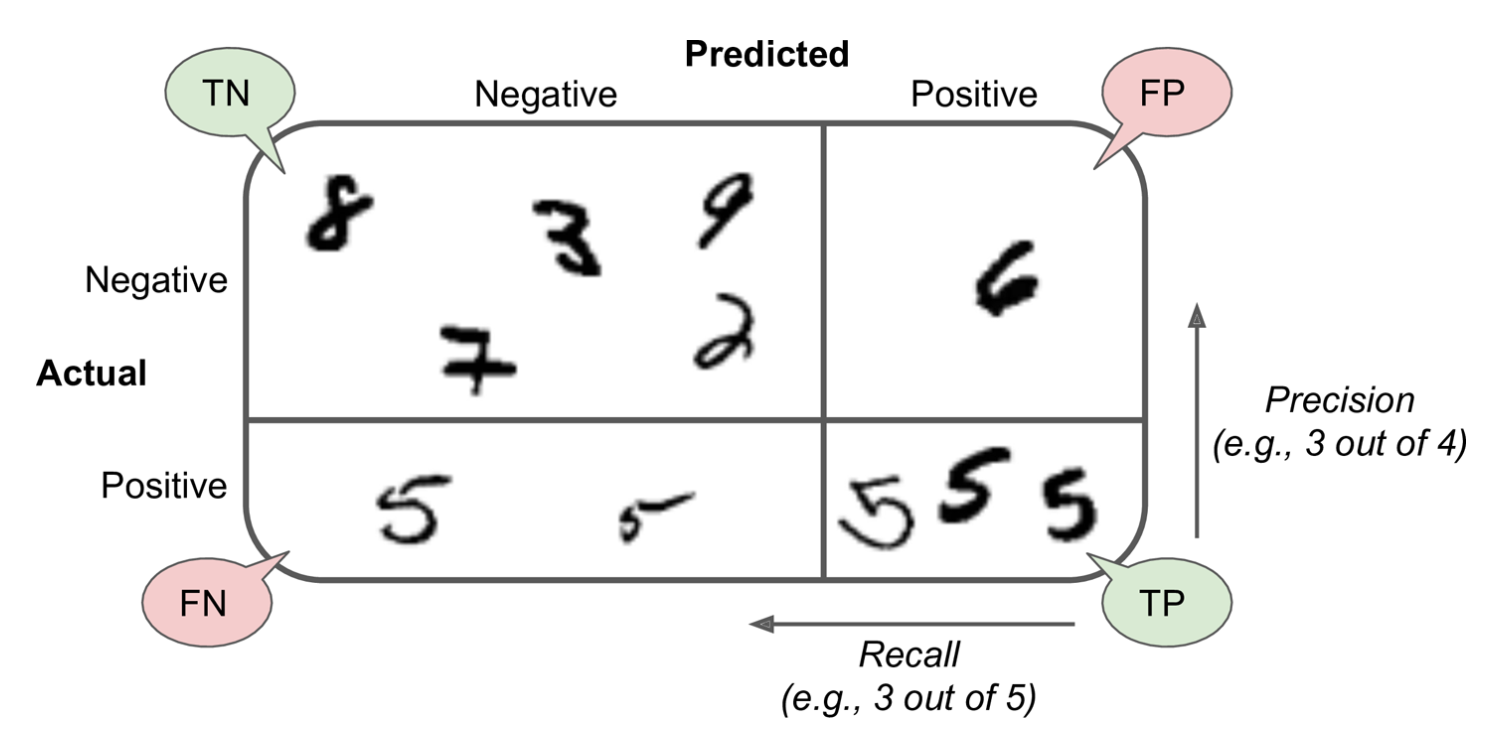
\includegraphics[scale=0.65]{Images/ConfusionMatrix.PNG}

\subsubsection*{Precision and Recall}

Scikit-Learn provides several functions to help compute classifier metrics, including precision
and recall. See below an example:

\pagebreak

\begin{minted}{python}
from sklearn.metrics import precision_score, recall_score

precision_score(y_train_5, y_train_pred) # == 4096 / (4096 + 1522)
# Output: 0.7291

recall_score(y_train_5, y_train_pred) # == 4096 / (4096 + 1325)
# Output: 0.7556
\end{minted}

\noindent
Now we can see that the classifier is definitely not as good as we originally thought. From 
\textbf{Precision}, we now see that when the classifier claims an image is of a 5, it is only 
correct about 72.9\% of the time. Additionally, from \textbf{Recall}, we can see that the classifier 
only detects 75.6\% of the 5s. \\

\noindent
In addition, we often find it useful to combine both precision and recall into a single metric which is 
known as the $\mathbf{F_{1} \textbf{ score}}$. This new metric can be defined as follows:

$$\mathbf{F_{1}} = \frac{2}{\frac{1}{\text{precision}} + \frac{1}{\text{recall}}} = 2 \times \frac{\text{Precision} \times \text{Recall}}{{\text{Precision}} + \text{Recall}} = \frac{\text{TP}}{\text{TP} + \frac{\text{FN} + \text{FP}}{2}}$$

\noindent
As follows, Scikit-Learn has a built in function for this as well. We can call \mintinline{python}{f1_score()}
function.

\begin{minted}{python}
from sklearn.metrics import f1_score
f1_score(y_train_5, y_train_pred)
# Output: 0.7421    
\end{minted}

\noindent
\textbf{Note}: that the $F_{1}$ score favors classifiers that have similar precision and recall. This may not 
always be that case that we want. Some cases may call for mostly caring about precision, and on other cases it 
may be best to only care a lot about recall. \\

\noindent
We can also not have both high precision and recall, as if we increase one the other tends to decrease. This is known
as the \textit{Precision/Recall Trade-Off}.

\subsubsection{ROC Curve}

The \textit{Revceiver Operating Characteristic} (ROC) curve is another common way to evaluate a binary classifiers
ability to predict correct classes. The ROC curve is created by plotting the \textit{True Positive Rate} (Also 
known as Recall) against the \textit{False Positive Rate} (FPR). The FPR is the ratio of negative instances that are
incorrectly classified as positive. It is also equal to $1 -$ the \textit{True Negative Rate} (TNR), which is the 
ratio of negative instances that are correctly classified as negative. TNR is also called \textit{Specificity}. \\

\noindent 
\textbf{Note}: As a general rule, it is better to use the \textit{Precision/Recall Curve} when the positive class is
rare or when we care more about the false positive than the false negatives. Otherwise, it is better to use the ROC
curve. 

\subsection{Multiclass Classifification}

In this section we will be discussing how we can train classifiers that are choosing between more than just 
two separate classes. Some algorithms (SGD classifiers, Random Forest Classifiers, and Naive Bayes Classifiers) are 
capable of handling multiple classes natively. However, others (Logisitc Regression, SVM) are strictly binary
classifiers, but as we will see, there are strategies so that we can perform multiclass classification with 
binary classifiers. \\

\noindent
There are 2 strategies for making it possible for binary classifiers to have the ability to classify multiple 
classes. The strategies are known as \textbf{One-Versus-Rest} (OvR) and \textbf{One-Versus-One} (OvO).

\subsubsection*{One-Versus-Rest}

This strategy is fairly basic in that, for example, if we want to train binary classifiers to classify digit images
into 10 classes (0 to 9), we can train 10 binary classifiers, one for each digit (0-detector, 1-detector, etc.). Then
when we want to classify an image, we get a decision score from each classifier for that image and we select the 
class whose classifier outputs the highest score.

\subsubsection*{One-Versus-One}

The second strategy is to train binary classifiers for every pair of digits to distinguish 0s and 1s, 0s and 2s, 
1s and 2s, and so on. If there are N classes then we will need to train $\frac{N(N-1)}{2}$ classifiers. For the 
MNIST data we will need to train 45 binary classifiers. When we want to classify an image, we have to run the image
through all 45 classifiers and see which class wins the most duels. The main advantage of this strategy is that each
classifier only needs to be trained on a part of the training set for the two classes it must distinguish. \\

\noindent
However, some algorithms, such as SVM, scale very poorly with size of the training set. Therefore, it is preferred that
these algorithm use the OvO strategy as it is faster to train several classifiers on small training sets than a few
on large training sets (Although in most cases for binary classifiers, OvR is preferred).



\section{Support Vector Machines}

\textit{Support Vector Machines} (SVM), are one of the most popular models in Machine Learning. SVMs are capable of 
performing linear or nonlinear classification, regression and outlier detection. In general, SVMs are particularly 
strong suited in classification tasks that include complex datasets that are small or medium sized, as they do 
not scale well into larger datasets.

\subsection{How SVMs Work}

In this section we will be covering the mechanics behind how SVMs make predictions and how their training algorithms
work. A few words on notations, the bias terms will be called \textit{b}, and the feature weights vector will be 
called $\vec{w}$. Additionally, no bias feature will be added to the input feature vectors.

\subsubsection*{Decision Function and Predictions}

A linear SVM classifier model predicts the class of a new instance $\vec{x}$ by simply computing the
decision function: $\vec{w}^{\intercal}\vec{x} + b = w_{1}x_{1} + \cdots + w_{n}x_{n} + b$. If the result is 
positive, the predicted class $\hat{y}$ is the positive class (1), and otherwisw it is the negative class (0).
Below will be the function for a Linear SVM classifer's predictions:

\[ \hat{y} = 
\begin{cases} 
    0 & \text{if } \vec{w}^{\intercal}\vec{x} + b < 0 \\
    1 & \text{if } \vec{w}^{\intercal}\vec{x} + b \geq 0
\end{cases}
\] \\

\noindent
The figure below will show the plot of the decision function. It is a 2D plane because the dataset we are 
training the model on has only 2 features: petal width and petal length (Iris Datset). The decision boundary
is the set of points where the decision function is equal to 0: it is the intersection of 2 planes, which 
is a straight line (represented by the thick solid line).

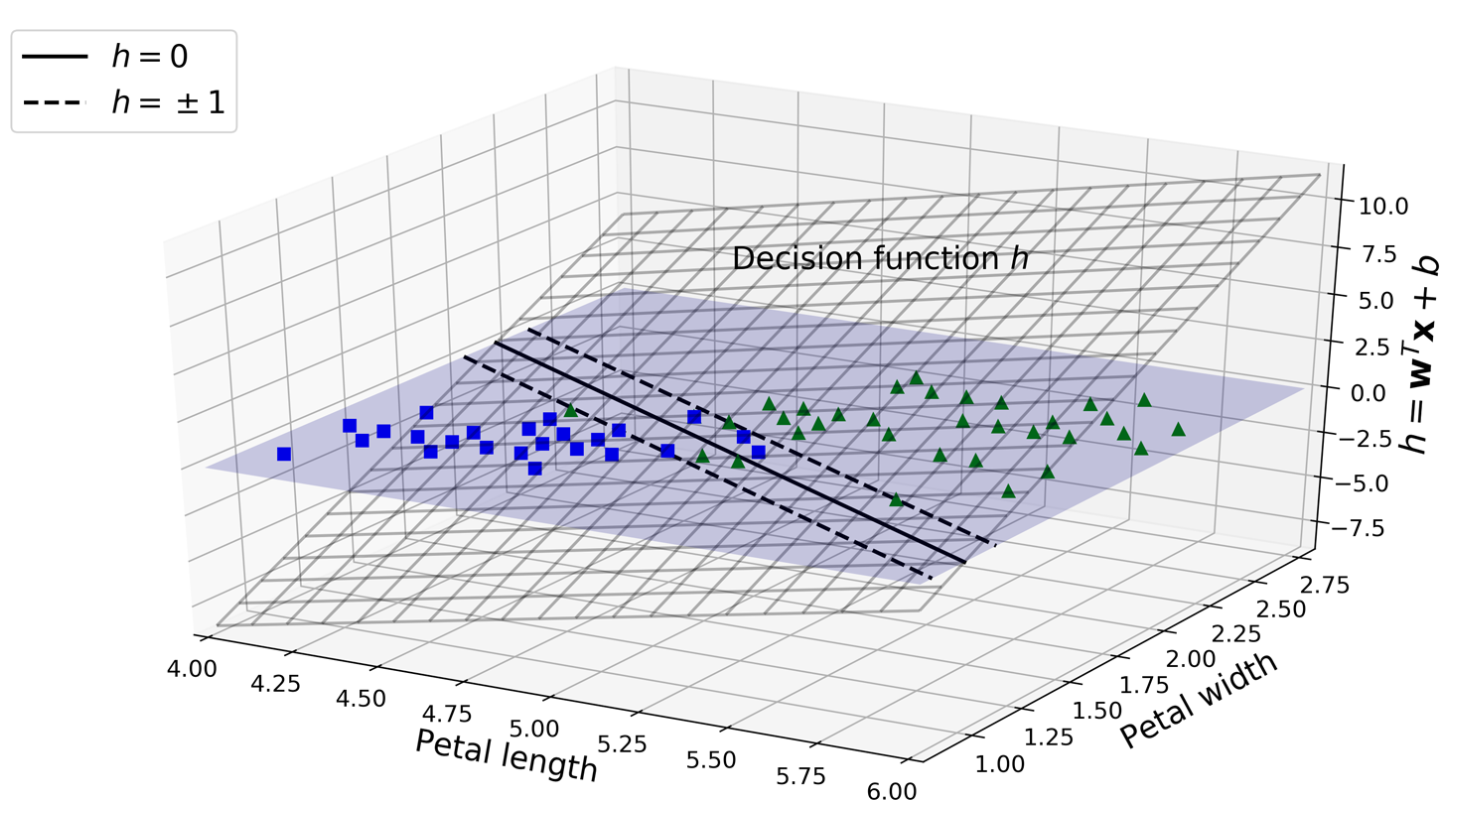
\includegraphics[scale=0.65]{Images/svm_DecisionFunc.PNG}

\noindent
The dashed lines represent the points where the decision function is equal to 1 or -1. \textbf{Note:}
they are parallel and at equal distance to the decision boundary, and they form a margin around
it. When we train a linear SVM classifier, we are finding the values of $\vec{w}$ and $b$ that 
make this margin as wide as possible while avoiding margin violations (\textit{hard margin}) 
or limiting them (\textit{soft margin}). 

\subsubsection*{Training Objective}

Consider the norm of the weight vector, $\norm{\vec{w}}$, we find that it is equivalent to the slope of the
decision function. If we were to divide this slope by 2, we will also find that the points where the decision
function is equal to $\pm 1$ are going to twice as far away from the decision boundary. This can be seen in the 
figure below:

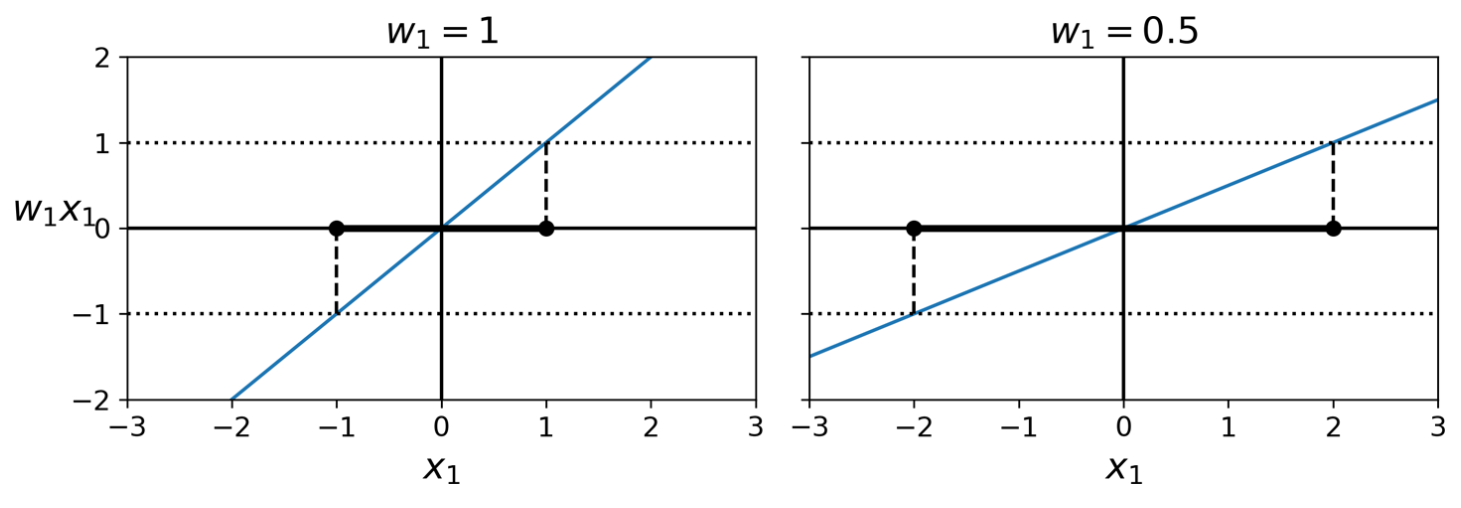
\includegraphics[scale=0.65]{Images/weightVec.PNG}

\noindent
Therefore, we want to minimize $\norm{\vec{w}}$ to get the largest possible margin. Additionally, if we want to
avoid any margin violations (hard margin), then we need the decision function to be greater than 1 for all 
positive training instances and lower than -1 for negative training instances. \\

\noindent
Further, if we define $t^{(i)} = -1$ for negative instance (if $y^{(i)} = 0$) and $t^{(i)} = 1$ for positive
instances (if $y^{(i)} = 1$), then we can express the constraint as $t^{(i)}(\vec{w}^{\intercal}\vec{x}^{(i)}+b) \geq 1$
for all instances.\\

\noindent
Finally, we can express the \textbf{hard margin} linear SVM classifier objective as the constrained optimization 
problem below:

\[
\begin{aligned}
\min_{\vec{w},b} \quad & \frac{1}{2}\vec{w}^{\intercal}\vec{w}\\
\textrm{subject to:} \quad & t^{(i)}(\vec{w}^{\intercal}\vec{x}^{(i)}+b) \geq 1 & \textrm{for } i = 1, 2, \cdots, m
\end{aligned}
\] \\

\noindent
\textbf{Note:} We are minimizing $\frac{1}{2} \vec{w}^{\intercal}\vec{w}$, which is just equal to 
$\frac{1}{2} \norm{\vec{w}}^{2}$, rather than minimizing $\norm{\vec{w}}$. This is because $\frac{1}{2} \norm{\vec{w}}^{2}$
has a nice derivative, which is just $\vec{w}$, whereas $\norm{\vec{w}}$ is not differentiable at $\vec{w} = 0$. 
In general optimization algorithms work much better on differentiable functions.\\

\noindent
For the \textbf{soft margin} objective, we need to a \textit{slack variable} $\zeta^{(i)} \geq 0$ for each 
instance. $\zeta^{(i)}$ can be described as how much the $i^{th}$ instace is allowed to violate the margin
(decision boundary). However, now we have two conflicting objectives:

\begin{itemize}
    \item First, is to minimize the slack variables as much as possible to reduce the margin violations
    \item Second, make $\frac{1}{2} \vec{w}^{\intercal}\vec{w}$ as small as possible to increase the margin
\end{itemize}

\noindent
Finally, this is where the \mintinline{python}{C} hyperparameter comes in. This hyperparameter allows us to 
define the tradeoff between these two objectives, thus, giving us the constrained optimization problem for 
the \textbf{soft margin} linear SVM classifier:

\[
\begin{aligned}
\min_{\vec{w},b, \zeta} \quad & \frac{1}{2}\vec{w}^{\intercal}\vec{w} + C\sum^{m}_{i=1} \zeta^{(i)}\\
\textrm{subject to:} \quad & t^{(i)}(\vec{w}^{\intercal}\vec{x}^{(i)}+b) \geq 1 - \zeta^{(i)} & \textrm{ for } i = 1, 2, \cdots, m\\
                           & \zeta^{(i)} \geq 0
\end{aligned}
\]

\subsubsection*{Quadratic Programming}

Hard and Soft Margin problems are both convex quadratic optimization problems with linear constraints. This is 
commonly known as \textit{Quadratic Programming} (QP) problems. There are many algorithms that can be used
for this task. Take a look at this \changeurlcolor{blue}\href{https://web.stanford.edu/~boyd/cvxbook/bv_cvxbook.pdf}{book} for more 
detailed explanations of these algorithms. \\

\noindent
The general Quadratic Programming problem to solve is given by:

\[
\begin{aligned}
\min_{\vec{p}} \quad & \frac{1}{2}\vec{p}^{\intercal}\vec{H}\vec{p} + \vec{f}^{\intercal}\vec{p}\\
\textrm{subject to:} \quad & \vec{A}\vec{p} \leq \vec{b} \\
\textrm{where} \quad & 
\begin{cases} 
    \vec{p} & \textrm{ is an } n_{p}-\textrm{dimensional vector } (n_{p} = \textrm{ number of parameters}) \\
    \vec{H} & \textrm{ is an } n_{p} \times n_{p} \textrm{ matrix} \\
    \vec{f} & \textrm{ is an } n_{p}-\textrm{dimensional vector} \\
    \vec{A} & \textrm{ is an } n_{c} \times n_{p} \textrm{ matrix } (n_{c} = \textrm{ number of constraints})\\
    \vec{b} & \textrm{ is an } n_{c}-\textrm{dimensional vector}
\end{cases}
\end{aligned}
\] \\

\noindent 
Note that the expression $\vec{A}\vec{p} \leq \vec{b}$ defines a $n_{c}$ constraints: $\vec{p}^{\intercal}\vec{a}^{(i)} \leq b^{(i)}$
for $i = 1, 2, \cdots, n_{c}$, where $\vec{a}^{(i)}$ is the vector containing the elements of the $i^{th}$ row
of $\vec{A}$ and $b^{(i)}$ is the $i^{th}$ element of $\vec{b}$.\\

\noindent 
As an example, we can verify the QP parameters for a hard margin linear SVM classifier below:

\begin{itemize}
    \item $n_{p} = n + 1$, where $n$ is the number of features (+1 is for the bias term)
    \item $n_{c} = m$, where $m$ is the number of training instances
    \item $\vec{H}$ is the $n_{p} \times n_{p}$ identity matrix, except with a zero in the top-left cell (to ignore the bias term)
    \item $\vec{f} = 0$, an $n_{p}-$dimensional vector full of 0s
    \item $\vec{b} = -1$, an $n_{c}-$dimensional vector full of -1s
    \item $\vec{a}^{(i)} = -t^{(i)}\dot{\vec{x}}^{(i)}$, where $\dot{\vec{x}}^{(i)}$ is equal to $\vec{x}^{(i)}$ with an extra bias feature $\dot{\vec{x}}_{0} = 1$
\end{itemize}

\noindent
Thus, one way to train a hard margin linear SVM classifier is to use an off-the-shelf QP solver and pass it the 
preceding parameters. The resulting vector $\vec{p}$ will contain the bias term $b = p_{0}$ and the feature 
weights $w_{i} = p_{i}$ for $i = 1, 2, \cdots, n$. Similarily, we can solve the soft margin problem using 
a QP solver as well. 

\subsubsection*{The Dual Problem}

For more indepth explanation of this problem reference \changeurlcolor{blue}\href{https://en.wikipedia.org/wiki/Duality_(optimization)}{this site}.\\

\noindent
In its most basic form the \textit{Dual Problem (Duality)} is when we have a given constrained optimization
problem, known as the \textit{primal problem}, and it is possible to express a different but closely related 
problem, called the \textit{dual problem}. Typically, the dual problem gives a lower bound to the solution of the 
primal problem. \\

\noindent
Fortunately, the SVM constrained optimization problem meets these conditions, so we have the choice to solve the 
primal or dual problem. The optimal solutions for both will be the same. To derive the unconstrained optimization
problem for the hard margin SVM, we need to use \textit{Lagrange Multipliers}. \\

\noindent
Given the constraints we shown earlier, we can write down the \textit{Generalized Lagrangian} for the hard margin
problem for linear SVMs. $\alpha^{(i)}$, is the variable that is called the \textit{Karush-Kuhn-Tucker} (KKT)
multipliers. Below will be the Lagrangian:

\[
\begin{aligned}
\mathcal{L}(\vec{w}, b, \alpha) = \frac{1}{2}\vec{w}^{\intercal}\vec{w} - \sum_{i=1}^{m} \alpha^{(i)}(t^{(i)}(\vec{w}^{\intercal}\vec{x}^{(i)} + b) - 1)\\
\textrm{with } \alpha^{(i)} \geq 0 \textrm{ for } i = 1, 2, \cdots, m
\end{aligned}
\]\\

\noindent
As follows with Lagrange multipliers, we can compute the partial derivatives and locate the optimal points. If
there is a solution, it will be among the stationary points $(\hat{\vec{w}}^{\intercal}, \hat{b}, \hat{\alpha})$ 
that respect the KKT Conditions:

\begin{itemize}
    \item Respect the problems constraints: $t^{(i)}(\vec{w}^{\intercal}\vec{x}^{(i)}+b) \geq 1 \textrm{ for } i = 1, 2, \cdots, m$
    \item Verify $\hat{\alpha}^{(i)} \geq 0 \textrm{ for } t = 1,2, \cdots, m$
    \item Either $\hat{\alpha}^{(i)} = 0$ or the $i^{th}$ constraint must be an \textit{active constraint}, meaning it
    must hold by equality: $t^{(i)}(\vec{w}^{\intercal}\vec{x}^{(i)}+b) = 1$. This condition is called the 
    \textit{complementrary slackness} condition. It implied that either $\hat{\alpha}^{(i)} = 0$ or the 
    $i^{th}$ instance lies on the boundary (it is a support vector).
\end{itemize}

\noindent 
\textbf{Note} that the KKT conditions are necessary conditions for a stationary point to be a solution of the 
constrained optimization problem. Fortunately, the SVM optimization problem meets all these conditions, so any
stationary point that meets the KKT conditions is guaranteed to be a solution to the constrained optimization 
problem.\\

\noindent
We can compute the partial derivatives of the generalized Lagrangian with regard to $\vec{w}$ and $b$:

$$\nabla_{\vec{w}} \mathcal{L}(\vec{w}, b, \alpha) = \vec{w} - \sum_{i=1}^{m} \alpha^{(i)}t^{(i)}\vec{x}^{(i)}$$

$$\frac{\partial}{\partial b}\mathcal{L}(\vec{w}, b, \alpha) = -\sum_{i=1}^{m} \alpha^{(i)}t^{(i)}$$

\noindent
We then set these partial derivatives equal to zero, and we can get the following:

$$\hat{\vec{w}} = \sum_{i=1}^{m} \hat{\alpha}^{(i)} t^{(i)} \vec{x}^{(i)}$$

$$\sum_{i=1}^{m} \hat{\alpha}^{(i)} t^{(i)} = 0$$

\noindent
Now we can plug these results into the definition of the generalized Lagrangian and we get the following dual 
problem form for the SVM problem:

\[
\begin{aligned}
\mathcal{L}(\hat{\vec{w}}, \hat{b}, \alpha) = \frac{1}{2} \sum_{i=1}^{m} \sum_{j=1}^{m} \alpha^{(i)} \alpha^{(j)} t^{(i)} t^{(j)} \vec{x}^{(i)\intercal} \vec{x}^{(j)} - \sum_{i=1}^{m} \alpha^{(i)} \\
\textrm{with } \alpha^{(i)} \geq 0 \textrm{ for } i = 1, 2, \cdots, m
\end{aligned}
\] \\

\noindent
We now want to find the vector $\hat{\vec{\alpha}}$, that minimizes this function, while $\hat{\alpha}^{(i)} \geq 0$
for all instances. \\

\noindent
Once we find the optimal $\hat{\vec{\alpha}}$, we can compute $\hat{\vec{w}}$ using the partial derivative w.r.t. 
$\vec{w}$ of the Lagrangian. To compute $\hat{b}$, we can use the fact that a support vector must satisfy 
$t^{(i)}(\hat{\vec{w}}^{\intercal}\vec{x}^{(i)}+\hat{b}) = 1$, so if the $k^{th}$ instance is a support vector
(i.e., $\hat{\alpha}^{(k)} > 0$), we can use it to compute $\hat{b} = t^{(k)} - \hat{\vec{w}}^{\intercal}\vec{x}^{(k)}$.
However, it is often preferred to compute the average over all support vectors to get a more stable and 
precise value as show below: (Bias term estimation using the dual form)

$$\hat{b} = \frac{1}{n_{s}} \sum_{\substack{i = 1 \\ \hat{\alpha}^{(i)}>0}}^{m} [t^{(i)} - \hat{\vec{w}}^{\intercal}\vec{x}^{(i)}]$$

\noindent
Altogether it is found that the dual problem is faster to solve than the primal one when the number of training
instances is smaller than the number of features. However, more importantly the dual problem allows us to use 
something called the \textit{kernel trick} prossible, while the primal does not (More explained in next section).

\subsubsection*{Kernelized SVMs}

Suppose we want to apply a second-degree polynomial transformation to a two-dimensional training set, then train a 
linear SVM classifier on the transformed training set. Below we can see the second-degree polynomial mapping 
function $\boldsymbol{\phi}$ we want to apply:

$$\boldsymbol{\phi}(\vec{x}) = 
\boldsymbol{\phi}
\begin{pmatrix}
    \begin{pmatrix}
        x_{1} \\
        x_{2}
    \end{pmatrix}
\end{pmatrix}
= 
\begin{pmatrix}
    x_{1}^{2} \\
    \sqrt{2}x_{1}x_{2} \\
    x_{2}^{2}
\end{pmatrix}
$$ \\

\noindent
\textbf{Notice:} that the transformed vector is 3D instead of 2D. Now we take a look at how 2D vectors, $\vec{a}$ and 
$\vec{b}$, if we apply this second-degree polynomial mapping and then compute the dot product of the transformed 
vectors we get the following:

\[
\begin{aligned}
\boldsymbol{\phi}(\vec{a})^{\intercal}\boldsymbol{\phi}(\vec{b}) = 
\begin{pmatrix}
    a_{1}^{2} \\
    \sqrt{2}a_{1}a_{2} \\
    a_{2}^{2}
\end{pmatrix}
^{\intercal}
\begin{pmatrix}
    b_{1}^{2} \\
    \sqrt{2}b_{1}b_{2} \\
    b_{2}^{2}
\end{pmatrix}
=
a_{1}^{2}b_{1}^{2} + 2a_{1}b_{1}a_{2}b_{2} + a_{2}^{2} b_{2}^{2}\\
= (a_{1}b_{1} + a_{2}b_{2})^{2} = 
\begin{pmatrix}
    \begin{pmatrix}
        a_{1}\\
        a_{2}
    \end{pmatrix}
    ^{\intercal}
    \begin{pmatrix}
        b_{1} \\
        b_{2}
    \end{pmatrix}
\end{pmatrix}
^{2} = 
(\vec{a}^{\intercal}\vec{b})^{2}
\end{aligned}
\]

\noindent
From the above, we can see that the dot product of the transformed vectors is equal to the sum of the square of the 
dot product of the original vectors 
$\boldsymbol{\phi}(\vec{a})^{\intercal}\boldsymbol{\phi}(\vec{b}) = (\vec{a}^{\intercal}\vec{b})^{2}$.\\

\noindent
\textbf{Key Insight:} if we want to apply the transformation $\boldsymbol{\phi}$ to all training instances, then
the dual problem (mentioned earlier), will be the dot product 
$\boldsymbol{\phi}(\vec{x}^{(i)})^{\intercal}\boldsymbol{\phi}(\vec{x}^{(j)})$. But if $\boldsymbol{\phi}$ is 
the second-degree polynomial transformation defined earlier, then we can replace this dot product of the 
transformed vectors simply by $(\vec{x}^{(i)\intercal}\vec{x}^{(j)})^{2}$. Therefore, we do not need to transform
the training instances at all; just replace the dot product by its square in the dual problem for SVM defined 
earlier. The following result will be the same as if we went through the trouble of transforming the training 
set then fitting a linear SVM algorithm, however, this "trick" makes the process much more computationally
efficient. \\

\noindent
In Machine Learning, a \textit{kernel} is a function capable of computing the dot product 
$\boldsymbol{\phi}(\vec{a}^{\intercal})\boldsymbol{\phi}\vec{b}$, based only on the original vectors $\vec{a}$ 
and $\vec{b}$, without having to compute (or even know) the transformation $\boldsymbol{\phi}$. Below will be a 
list of some of the most commonly used kernels:

\[
\begin{aligned}
\textrm{Linear:} \quad & K(\vec{a}, \vec{b}) = \vec{a}^{\intercal}\vec{b} \\
\textrm{Polynomial:} \quad & K(\vec{a}, \vec{b}) = (\gamma\vec{a}^{\intercal}\vec{b} + r)^{d} \\
\textrm{Gaussian RBF:} \quad & K(\vec{a}, \vec{b}) = \textrm{exp}(-\gamma \norm{\vec{a} - \vec{b}}^{2}) \\
\textrm{Sigmoid:} \quad & K(\vec{a}, \vec{b}) = \textrm{tanh}(\gamma\vec{a}^{\intercal}\vec{b} + r)
\end{aligned}
\] \\

\noindent
\textbf{Mercer's Theorem:} According to this theorem if a function $K(\vec{a}, \vec{b})$ respects a few 
mathematical conditions called \textit{Mercer's Conditions} (e.g., K must be continous and symmertric in its 
arguements so that $K(\vec{a}, \vec{b}) = K(\vec{b}, \vec{a})$, etc.), then there exists a function 
$\boldsymbol{\phi}$ that maps $\vec{a}$ and $\vec{b}$ into another space (possible with much higher dimensions) 
such that $K(\vec{a}, \vec{b}) = \boldsymbol{\phi}(\vec{a})^{\intercal} \boldsymbol{\phi}(\vec{b})$. We can use 
K as a kernel because we know that $\boldsymbol{\phi}$ exists, even if we dont know exactly what 
$\boldsymbol{\phi}$ is. For example int he case of the Gaussian RBF kernel, it can be shown that 
$\boldsymbol{\phi}$ maps each training instance to an infinite-dimensional space.\\

\noindent
Note, that some frequently used kernels (such as the sigmoid kernel) do not respect all of the Mercer's conditions,
yet they generally work well in practice. \\

\noindent
Earlier in this section we covered how to get to the dual solution to the primal solution in the case of the 
linear SVM classifier. But if we were to apply the kernel trick, we will end up with equations that include
$\boldsymbol{\phi}(x^{(i)})$, which may be large or even infinite, so we are not able to compute it. Then we 
ask the question how can we make predictions without knowing $\vec{\hat{w}}$? Well we can plug in $\vec{\hat{w}}$
from the partial derivatives we took earlier, into the decision function for a new instance $\vec{x}^{(n)}$, and
we get an equation with only dot products between input vectors. This is what makes it possible to use the kernel
trick. Below will be how we make predictions with a kernelized SVM:

\begin{eqnarray}
h_{\vec{\hat{w}}, \vec{\hat{b}}}\left(\boldsymbol{\phi}(\vec{x}^{n})\right) &=& \vec{\hat{w}}^{\intercal}\boldsymbol{\phi}\left(\vec{x}^{(n)}\right) + \hat{b} =\left(\sum_{i=1}^{m} \hat{\alpha}^{(i)}t^{(i)}\boldsymbol{\phi}\left(\vec{x}^{(i)}\right)\right)^{\intercal}\boldsymbol{\phi}\left(\vec{x}^{(n)}\right) + \hat{b} \nonumber \\
                                                                 &=& \sum_{i=1}^{m} \hat{\alpha}^{(i)}t^{(i)} \left(\boldsymbol{\phi}\left(\vec{x}^{(i)}\right)^{\intercal}\boldsymbol{\phi}\left(\vec{x}^{(n)}\right)\right) + \hat{b} \nonumber \\
                                                                 &=& \sum_{\substack{i=1 \\ \hat{\alpha}^{(i)} > 0}}^{m} \hat{\alpha}^{(i)} t^{(i)} K\left(\vec{x}^{(i)}, \vec{x}^{(n)}\right) + \hat{b} \nonumber
\end{eqnarray}

\noindent
Note that since $\alpha^{(i)} \neq 0$ only for support vectors, making predictions involves computing the dot
product of the new input vector $\vec{x}^{(n)}$ with only the support vectors, not all the training instances.
Additionally, we will use the same trick to compute the bias term $\hat{b}$:

\begin{eqnarray}
\hat{b} &=& \frac{1}{n_{s}} \sum_{\substack{i=1 \\ \hat{\alpha}^{(i)} > 0}}^{m} \left(t^{(i)} - \vec{\hat{w}}^{\intercal}\boldsymbol{\phi}\left(\vec{x}^{(i)}\right)\right) \nonumber \\
        &=& \frac{1}{n_{s}} \sum_{\substack{i=1 \\ \hat{\alpha}^{(i)} > 0}}^{m} \left(t^{(i)} - \left(\sum_{j=1}^{m} \hat{\alpha}^{(j)}t^{(j)}\boldsymbol{\phi}\left(\vec{x}^{(j)}\right)\right)^{\intercal} \boldsymbol{\phi}\left(\vec{x}^{(i)}\right)\right) \nonumber \\
        &=& \frac{1}{n_{s}} \sum_{\substack{i=1 \\ \hat{\alpha}^{(i)} > 0}}^{m} \left(t^{(i)} - \sum_{\substack{j=1 \\ \hat{\alpha}^{(j)}}}^{m} \hat{\alpha}^{(j)}t^{(j)} K\left(\vec{x}^{(i)}, \vec{x}^{(j)}\right)\right) \nonumber
\end{eqnarray}

\noindent
Finally, we have finished understanding the inner workings of the kernelized SVM. 

\subsection{Linear SVM Classification}
The fundamental idea behind \textit{Support Vector Machines} is to find a line that can separate two separate 
classes (Data would be known as \textit{linearly separable}). The goal of a SVM classifier is to find a way to 
separate the two classes, but to simultaneously also fit the widest possible street for separating the two 
classes. This is called \textit{Large Margin Classification}.\\

\noindent
\textbf{Note:} adding more training instaces that are "off the street" will not affect the decision boundary at
all. The decision boundary is determined (or "supported) by the instances located on the edge of the street only. 
These instances are called the \textit{support vectors}. \\ 

\noindent
\textbf{Important}, SVMs are sensitive to feature scaling, so we must be wary when we are training models on 
unscaled data or when we are doing any feature engineering.

\subsubsection{Hard Margin Classification}

\textit{Hard Margin Classification} is when we are looking to very strict with the classification of our instances.
We can impose a rule there all instances must be off the decision boundary and on the right side. This is the 
basic rule of hard margin classification. \\

\noindent
However there are two main issues that are associated with this type of classification:

\begin{itemize}
    \item This type of classification \textbf{only} works if the data is linearly separable.
    \item Training a model like this is also very sensitive to outliers. For example, with just one outlier 
    on the wrong side of the class will make it impossible for there to be a hard margin. This will also likely
    lead to having the model generalize very poorly.     
\end{itemize}

\noindent
Therefore, in most cases it is not preferred to use hard margin classification when training a SVM as it is not
able to handle many real world datasets.

\subsubsection{Soft Margin Classification}

On the other hand, \textit{Soft Margin Classification} is a much more flexible classification system. Here the 
objective is to find the right balance between keeping the decision boundary as large as possible and limiting the 
\textit{margin violations} (i.e., instances that end up in the middle of the boundary or on the wrong side). \\

\noindent
When creating a SVM model using Scikit-Learn, there is a hyperparameter \mintinline{python}{C} that allows us to 
regularize the model. If we set a low value for \mintinline{python}{C}, then we end up with a more flexible model,
whereas, if we set a high \mintinline{python}{C}, then we get a model that much more similar to 
\textit{hard margin classification}.

\subsubsection*{Example of SVM in Python}

The following code will be using Scikit-Learn to train a linear SVM model on the iris dataset. The code will scale 
the features and then train the model. The objective of this model it to detect \textit{Iris Virginica} flowers in
the iris dataset. 

\begin{minted}{python}
import numpy as np
from sklearn import datasets
from sklearn.pipeline import Pipeline
from sklearn.preprocessing import StandardScaler
from sklearn.svm import Linear SVC

iris = datasets.load_iris() # Iris Dataset
X = iris["data"][:, (2, 3)] # Petal Length, Petal Width
y = (iris["target"] == 2).astype(np.float64) # Iris Virginica

svm_clf = Pipeline([
            ("Scaler", StandardScaler()),
            ("linear_svc", LinearSVC(C=1, loss="hinge")),
    ])

svm_clf.fit(X, y)

svm_clf.predict([[5.5, 1.7]])
# Output: array([1.])
\end{minted}

\noindent
Additionally, instead of using the \mintinline{python}{LinearSVC} class, we can also use the \mintinline{python}{SVC}
class with a linear kernel. When creating the SVC model, we will just need to specify \mintinline{python}{SVC(kernel="linear", C=1)}.

\subsection{Non-Linear SVM Classification}

There are many times when datasets are not anywhere close to being linearly separable. In this section we will be covering different
ways to go about creating nonlinear SVM classifiers. The first approach is to add more features, such as polynomial features, which
in some cases may lead to the dataset being linearly separable. As an example below we have 2 graphs, on the left there is just one 
variable, $x_{1}$, and we can clearly see that the data is not linearly separable. Now on the right graph, we add a second feature
$x_{2} = (x_{1})^{2}$, resulting in a 2D dataset that is perfectly linearly separable. \\

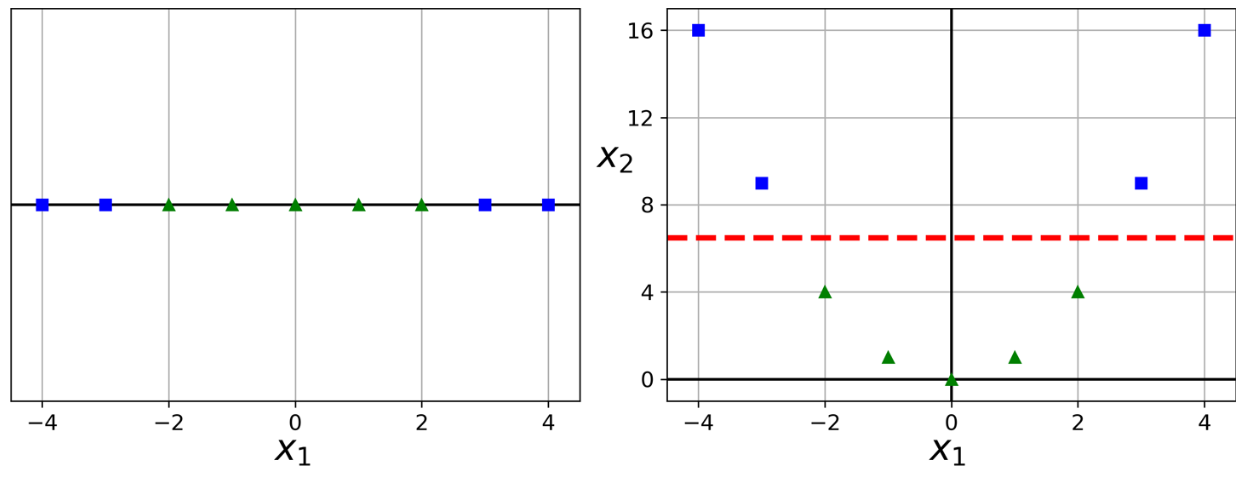
\includegraphics[scale=0.45]{Images/linearSeparable.PNG}

\noindent
To implement this using Scikit-Learn, we can create a \mintinline{python}{Pipeline} containing \mintinline{python}{PolynomialFeatures}
transformer, followed by a \mintinline{python}{StandardScaler} and a \mintinline{python}{LinearSVC}. The example below will be used 
on the moons dataset: this is a toy dataset for binary classification in which the data points are shaped as two interleaving 
half circles. Below will be the code:

\begin{minted}{python}
from skelarn.datasets import make_moons
from sklearn.pipeline import Pipeline
from sklearn.preprocessing import PolynomialFeatures, StandardScaler

X, y = make_moons(n_samples=100, noise=0.15)
polynomial_svm_clf = Pipeline([
        ("poly_features", PolynomialFeatures(degree=3)),
        ("scaler", StandardSCaler()),
        ("svm_clf", LinearSVC(C=10, loss="hinge"))
    ])

polynomial_svm_clf.fit(X, y)
\end{minted}

\noindent
Additionally, below we can see what the decision boundary of the polynomial SVM classifier looks like on the moons dataset.\\

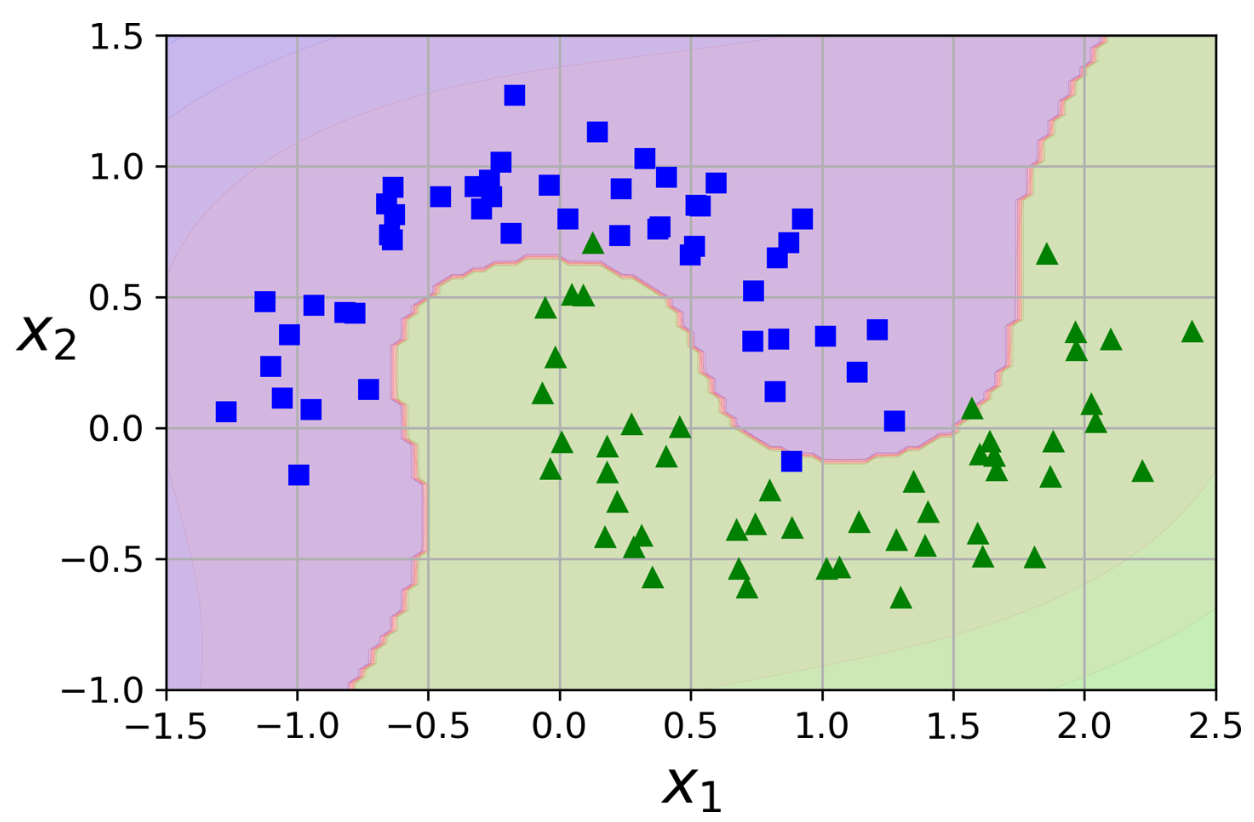
\includegraphics[scale=0.4]{Images/nonlinearSVM.PNG}

\subsubsection{Polynomial Kernel}

As seen above adding polynomial features is simple and quite easy to implement. However, at a low polynomial degree, this method does
not have the ability to deal with very complex datasets, and with high degree polynomials it creates a huge number of features 
making model training too slow. \\

\noindent
Fortunately, for SVMs, we can use the \textit{kernel trick}. As explained earlier, this trick makes it possible to get the same result
as if we had added many polynomial features, without having to actually add them into the model. This trick is already built into the 
\mintinline{python}{SVC} class. Below will be testing it on the moons dataset:

\begin{minted}{python}
from sklearn.svm import SVC
poly_kernel_svm_clf = Pipeline([
        ("scaler", StandardScaler()),
        ("svm_clf", SVC(kernel="poly", degree=3, coef0=1, C=5))
    ])

poly_kernel_svm_clf.fit(X, y)
\end{minted}

\noindent
In the code above, we are training a polynomial SVM using the kernel trick. Specifically in this case, we are training a 3-degree 
polynomial SVM classifier.\\

\noindent
In the graphic below, we can see the 3-degree polynomial
model on the left and on the right there is another 10-degree polynomial kernel. The hyperparameter \mintinline{python}{coef0} controls
how much the model is influenced by high-degree polynomials versus low-degree polynomials.\\

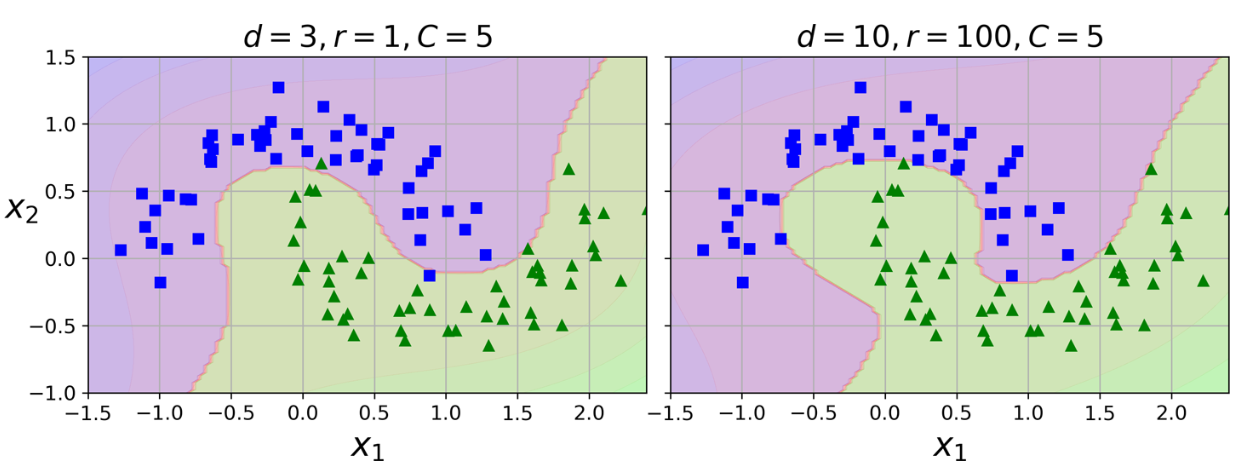
\includegraphics[scale=0.45]{Images/polyKernel.PNG}

\noindent
\textbf{Note:}, generally it is common practice to use grid search when trying to find the right hyperparameter values. It is fastest to 
first do a very coarse grid search, and then a finer grid search around the best values found. 

\subsubsection{Gaussian RBF Kernel}

Once again we can use the \textit{kernel trick} to reduce the computational expensiveness to compute all the additional features if we 
were to add all the similarity features manually. Below will be the implementation of \mintinline{python}{SVC} class with the 
Gaussian RBF Kernel:

\begin{minted}{python}
rbf_kernel_svm_clf = Pipeline([
        ("scaler", StandardScaler()),
        ("svm_clf", SVC(kernel="rbf", gamma=5, C=0.001))
    ])

rbf_kernel_svm_clf.fit(X, y)
\end{minted}

\noindent
Below will be a graphic showing different decision boundaries of the Gaussian RBF Kernel for varying values of \mintinline{python}{gamma}
($\gamma$) and \mintinline{python}{C}. Increasing \mintinline{python}{gamma} makes the bell-shaped curve narrower. As a result, each
instance's range of influence is smaller, in other words, the decision boundary ends up being more irregular, wiggling around individual
instances. Conversely, a small \mintinline{python}{gamma} value makes the bell-shaped curve wider, therefore, instances have a larger
range of influence, and the decision boundary ends up smoother. So $\gamma$ acts like a regularization hyperparameter: if we have a model
that is overfitting, we should reduce $\gamma$ and if it is underfitting, we should increase $\gamma$. \\

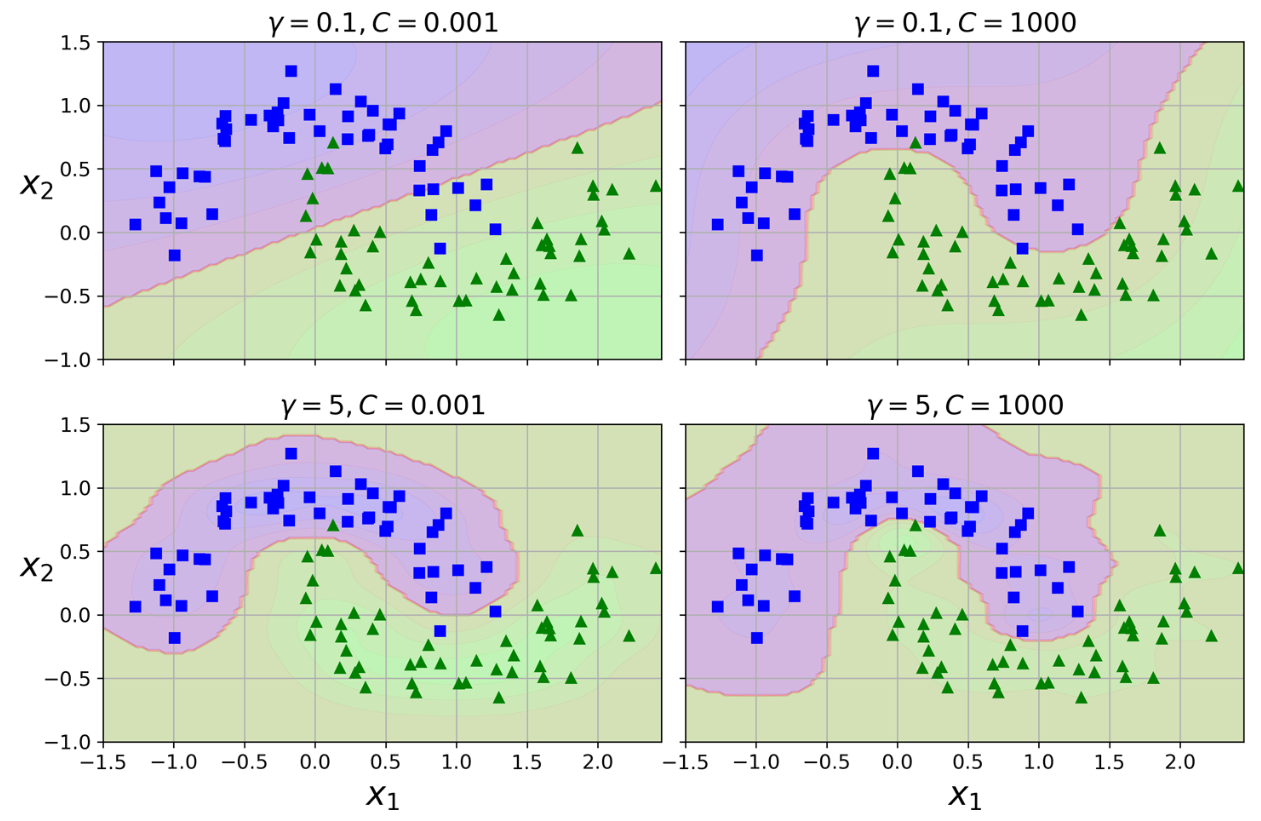
\includegraphics[scale=0.45]{Images/rbfKernel.PNG}

\noindent
There are other kernels that exist as well, but are used much more rarely. Some kernels are for specific data structures. For example, 
\textit{String Kernels} are sometimes used when classifiying documents or DNA sequences (e.g., using the \textit{string subsequence kernel}
or kernels based on the \textit{Levenshtein distance}).\\

\noindent
\textbf{As a Tip:}, one should always try the linear kernel first (remember that \mintinline{python}{LinearSVC} is much faster than 
\mintinline{python}{SVC(kernel="linear")}), especially is the training set is very large or if it has many features. Additionally, we can 
also try the Gaussian RBF kernel is the training set is not too large. Finally, it is never a bad idea to try and use a kernel specialized
whatever data structure that the training set may have.


\section{Decision Trees}

\textit{Decision Trees} are a versatile Machine Learning algorithm, that can outperform both classification and regression tasks,
and even multioutput tasks. This algorithm is very powerful, and is capable of fitting very complex datasets. Decision Trees
are also the fundamental building blocks of a Random Forest algorithm (Covered next section), which is one of the most 
powerful machine learning algorithms available today. \\

\noindent
In this section, we will cover how to train, visualize, and make predictions with Decision Trees (Using both Regression and 
classification).

\subsection{Training and Visualize a Decision Tree}

One of the easiest ways to understand \textit{Deicision Trees} is to build one and take a look how it makes predictions. Below
will be some code that trains a \mintinline{python}{DecisionTreeClassifier} on the iris dataset in Scikit-Learn:

\begin{minted}{python}
from sklearn.datasets import load_iris
from sklearn.tree import DecisionTreeClassifier

iris = load_iris()
X = iris.data[:, 2:] # Petal length and width
y = iris.target

tree_clf = DecisionTreeClassifier(max_depth=2, random_state=42)
tree_clf.fit(X, y)    
\end{minted}

\noindent
After running this code we can then visualize the Decision Tree by a graph format shown below:

\begin{center}
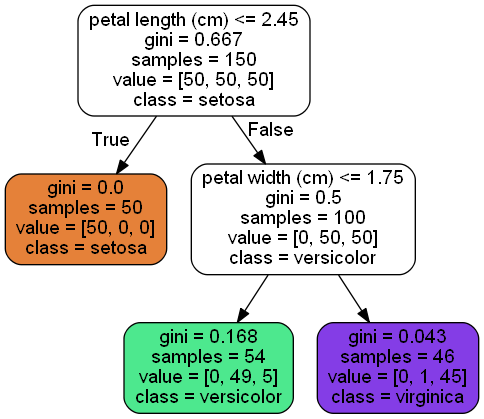
\includegraphics[scale=0.45]{Images/iris_tree.png}
\end{center}

\subsection{Making Predictions}

From the tree above we can show a logical process to classifying an iris flower. \\

\noindent
For example, lets say that we find an iris flower and we want to classify it, the steps will be as follows:

\begin{itemize}
    \item First we start at the \textit{root node} (depth 0, at the top): this node asks whether the flower's petal length is smaller than 
    2.45 cm.
    \item Second, if it is, then we move down to the root's left child node (depth 1, left)
    \item Third, we notice that in this case, this is a \textit{leaf node} (i.e., does not have any child nodes), so it is able to predict 
    the class of the iris. Which in this case, case classifies the iris flower as an \textit{iris setosa}
\end{itemize}

\noindent
**Note:** One of the great qualities about Decision Trees is that they require very little data preparation. I.e., they do not require 
feature scaling or centering at all. \\

\noindent
Node's Attributes:

\begin{itemize}
    \item \mintinline{python}{samples} attribute counts how many training instances it applies to. For example, 100 training instances
    have a petal length greater than 2.45 cm (depth 1, right), and of those 100, 54 have a petal width smaller than 1.75 cm 
    (depth 2, left). 
    \item \mintinline{python}{value} attribute tells us how many training isntances of each class this node applies to: for example, 
    the bottom-right node applies to 0 \textit{iris setosa}, 1 \textit{iris versicolor}, and 45 \textit{iris virginica}.
    \item \mintinline{python}{gini} attribute measures the \textit{impurity}: a node is "pure" (\mintinline{python}{gini=0}) if all 
    training instances it applies to belong to the same class. For example, since the depth-1 left node applies to only 
    \textit{iris setosa} training instances, it is pure and its gini score is 0. 
\end{itemize}

\noindent
Below will be the equation to compute the Gini Score:

$$G_{i} = 1 - \sum_{k=1}^{n} p_{i,k}^{2}$$

\noindent
In the equation above, $p_{i,k}$, is the ratio of class \mintinline{python}{k} instances among the training instances in the 
$i^{th}$ node \\

\noindent
Where we can compute the depth-2 left node gini attribute by the following: 

$$1 - \left(\frac{0}{54}\right)^{2} - \left(\frac{49}{54}\right)^{2} - \left(\frac{5}{54}\right)^{2} \approx 0.168$$ \\

\noindent
We can also view the decision boundaries of this Decision Tree through plots made in \mintinline{python}{matplotlib}. 

\begin{center}
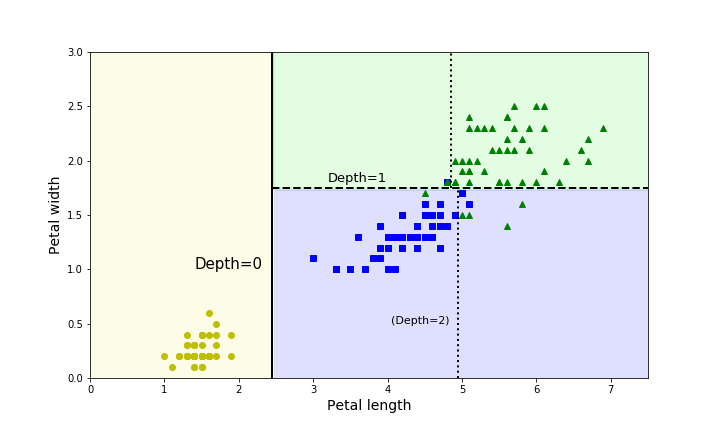
\includegraphics[scale=0.45]{Images/DecisionTreePlot.png}
\end{center}

\subsection{Estimating Class Probabilities}

A Decision Tree can also estimate the probability that an instance belongs to a particular class $k$. First it traverses the tree to find 
the leaf node for this instance, and then it returns the ration of training instances of class $k$ in this node. For example, suppose you 
have found a flower whose petals are 5 cm long and 1.5 cm wide. The corresponding leaf node is the depth-2 left node, so the Decision Tree 
should output the following probabilities: 0\% for Iris setosa ($\frac{0}{54}$), 90.7\% for Iris versicolor ($\frac{49}{54}$), and 9.3\% 
for Iris virginica ($\frac{5}{54}$). And if you ask it to predict the class, it should output Iris versicolor (class 1) because it has the 
highest probability. \\ 

\noindent
We can verify this with the following code:

\begin{minted}{python}
tree_clf.predict_proba([[5, 1.5]])
'''
Output:
array([[0.        , 0.90740741, 0.09259259]])
'''

tree_clf.predict([[5, 2.5]])
'''
Output:
array([1])
'''    
\end{minted}

\subsection{The CART Training Algorithm}

Scikit-Learn uses the \textit{Classification and Regresstion Tree} (CART) algorithm to train Decision Trees. This algorithm works by 
first splitting the training set into two subsets using a single feature $k$ and a threshold $t_{k}$ (e.g., "Petal Length $leq$ 2.45 cm).
It chooses $k$ and $t_{k}$ by searching for the pair $(k, t_{k})$ that produces the "purest" subsets (weighted by their size). The function
for this can be seen below:

\[
\begin{aligned}
 \quad & \vec{J}(k, t_{k}) = \frac{m_{left}}{m} G_{left} + \frac{m_{right}}{m} G_{right}\\
\textrm{where} \quad & 
\begin{cases} 
    G_{\text{left/right}} & \text{Measures the impurity of the left/right subset} \\
    m_{\text{left/right}} & \text{Is the number of instances in the left/right subset}
\end{cases}
\end{aligned}
\] \\

\noindent
Once the CART algorithm has sucessfully split the trianing set in two, it splits the subsets using the same logic then the sub-subsets, 
and so on. The algorthm stops either when it reaches the maximum depth defined by the modeller, or if it cannot find a split in the 
subset of data that will reduce the impurity. \\

\noindent
\textbf{Warning:} It is important to know that the CART algorithm is a \textit{greedy algorithm}, i.e., it will greedily search for an
optimum split at the top level, and then repeats the process at each subsequent level. It \textbf{DOES NOT} check whether or not thye 
split will lead to the lowest possible impurity several levels down. A greedy algorithm often produces a solution that's reasonably good 
but not guaranteed to be optimal. (Note that finding the optimal tree is known to be an \textit{NP-Complete} problem, which is why we 
must settle with a "reasonably good" solution.)

\subsection{Gini Impurity or Entropy?}

In Scikit-Learn, the Gini impurity is the default measure used in training Decision Tree Classifiers. However, we do have the option to select
\textit{entropy}, which is done by setting the \mintinline{python}{criterion} hyperparameter in a \mintinline{python}{DecisionTreeClassifier}
to \mintinline{python}{"entropy"}. Entropy has a similar meaning to the Gini impurity, in that, if entropy is zero for a given set, then all
instances in that set belong to the same class. Entropy can be calculated using the equation below:

$$H_{i} = - \sum_{\substack{k=1 \\ p_{i,k} \neq 0}}^{n} p_{i,k} log_{2} (p_{i,k})$$

\noindent
In most cases the deicison between using Entropy vs. Gini impurity does not make a big difference: they tend to usually lead to having similar
trees. Gini impurity is slightly faster to compute, so it tends to be a better default in that sense. In the cases when these two methods do tend
to differ, Gini impurity tends to isolate the most frequent class in its own branch of the tree, while entropy tends to produce slightly more
balanced trees.

\subsection{Regularization Hyperparameters}

It is important to know that Decision Trees do make many assumptions about the training data (as opposed to linear models (i.e., assume data 
is linear)). Therefore, if Decision trees are left unconstrained the tree structure will adapt itself to the training data, and likely severly
overfit it. \\

\noindent
Such a model with these type of traits are called \textit{nonparametric models}, not because the model itself does not have any parameters, but
because the number of parameters is not determined prior to training, so the model structure is free to stick closely to the data. On the other
hand, a \textit{parametric model}, such as a linear model, has a predetermined number of parameters, so its degree of freedom is limited, 
reducing the risk of overfitting (but also increasing the risk of underfitting). \\

\noindent
To reduce the risk of overfitting the training data, we need to restrict the Decision Tree's freedom during training. The regularization
hyperparameters depend on the algorithm used, but generally we can at least restrict the maximum depth of the Decision Tree. In Scikit-Learn,
this is controlled by the \mintinline{python}{max_depth} hyperparameter (The default is \mintinline{python}{None}, which means unlimited). 
Reducing \mintinline{python}{max_depth} will regularize the model and thus reduce the risk of overfitting. \\

\noindent
The \mintinline{python}{DecisionTreeClassifer} class has a few other parameters that similarly restrict the shape of the Decision Tree. These 
other hyperparameters will be listed below:

\begin{itemize}
    \item \mintinline{python}{min_samples_split}: The minimum number of samples a node must have before it can split
    \item \mintinline{python}{min_samples_leaf}: The minimum number of samples a leaf node must have
    \item \mintinline{python}{min_weight_fraction_leaf}: Same as \mintinline{python}{min_samples_leaf} but expressed as a fraction of the total
    number of weighted isntances
    \item \mintinline{python}{max_leaf_nodes}: The maximum number of leaf nodes
    \item \mintinline{python}{max_features}: The maximum number of features that are evaluated for splitting at each node
\end{itemize}

\noindent
\textbf{NOTE:} Other algorithms work by first training the Decision Tree without restrictions, then \textit{pruning} (deleting) unnecessary 
nodes. A node whose children are all leaf nodes is considered unnecessary if the purity improvement it provides is not statistically significant.
Standard statistcal tests, such as the $\chi^{2}$ test (chi-squared test), are used to estimate the probability that the improvement is purely
a result of chance (which is called the \textit{null hypothesis}). If the p-value, is higher than a given threshold (typically 5\%, controlled
by a hyperparameter), then the node is considered unnecessary and its children are deleted. the pruning continues until all unnecessary nodes
have been pruned.\\

\noindent
Finally, below will be an example of an unrestricted Decision tree and regularized Decision tree on the moons dataset in Scikit-Learn. We can see
that the model that does not have any regularization will have a much harder time generalizing as compared to the model with regularization.

\begin{center}
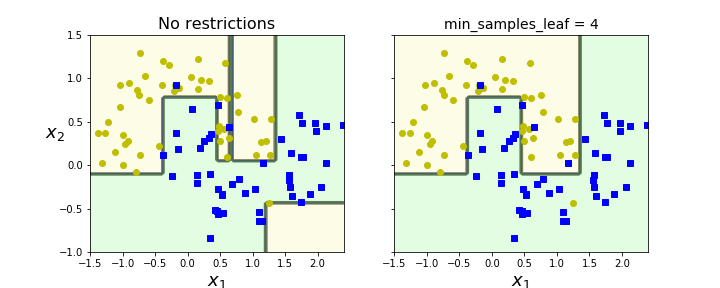
\includegraphics[scale=0.55]{Images/min_samples_leaf_plot.png}
\end{center}

\subsection{Regression}

Decision Trees are capable of performing regression tasks as well. Below we will use Scikit-Learn's \mintinline{python}{DecisionTreeRegressor}
class, training it on a noisy quadratic dataset with a \mintinline{python}{max_depth=2}:

\begin{minted}{python}
from sklearn.tree import DecisionTreeRegressor

# Quadratic training set + noise
np.random.seed(42)
m = 200
X = np.random.rand(m, 1)
y = 4 * (X - 0.5) ** 2
y = y + np.random.randn(m, 1) / 10

tree_reg = DecisionTreeRegressor(max_depth=2, random_state=42)
tree_reg.fit(X, y)
\end{minted}

\noindent
The resulting tree can be seen below:

\begin{center}
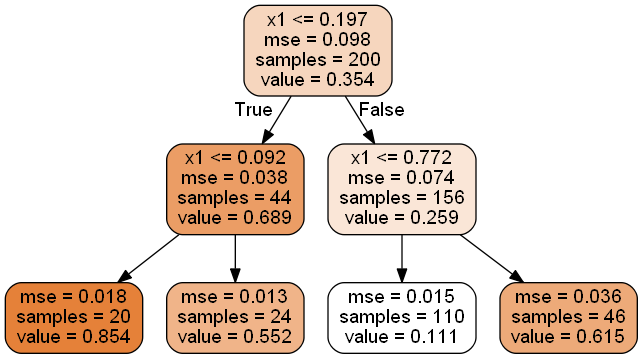
\includegraphics[scale=0.45]{Images/iris_tree_reg.png}
\end{center}

\noindent
We can see that the regression tree looks very similar to the tree that we built earlier. The main difference now is that instead of predicting 
a class in each node, we are now predicting a value instead. Additionally, we can use the same strategy as before when traversing the 
classification based tree (For example, if we wanted to find the node for an input value of $x_{1} = 0.6$). \\

\noindent
This model’s predictions are represented on the left in figure below. If you set \mintinline{python}{max_depth=3}, you get the predictions 
represented on the right. Notice how the predicted value for each region is always the average target value of the instances in that region. 
The algorithm splits each region in a way that makes most training instances as close as possible to that predicted value.

\begin{center}
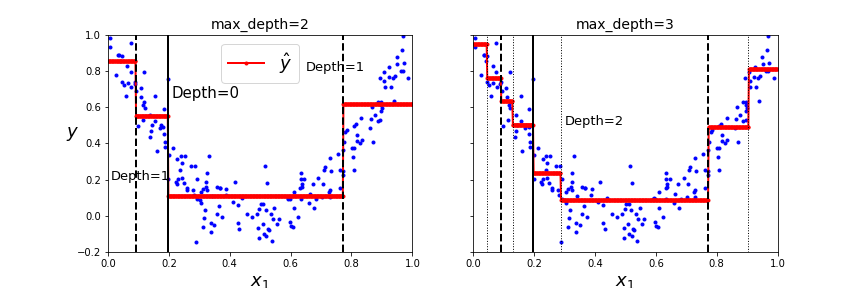
\includegraphics[scale=0.45]{Images/tree_regression_plot.png}
\end{center}

\noindent
The CART algorithm works similarly, except that instead of trying to split the training set in a way that minimizes impurity, it tries to split
the training set in a way that minimizes the \textit{mean squared error} (MSE). Below will be the cost function that the CART algorithm tries
to minimize:

\begin{equation*}   
\begin{aligned}
    \quad & \vec{J}(k, t_{k}) = \frac{m_{left}}{m} \text{MSE}_{left} + \frac{m_{right}}{m} \text{MSE}_{right}\\
\textrm{where} \quad & 
\begin{cases} 
    \text{MSE}_{\text{node}} = \sum_{i \in \text{node}} \left(\hat{y}_{node} - y^{(i)}\right)^{2} \\
    \hat{y}_{\text{node}} = \frac{1}{m_{\text{node}}} \sum_{i \in \text{node}} y^{(i)}
\end{cases}
\end{aligned}
\end{equation*}

\noindent
Additionally, just like classification tasks, Decision Trees are prone to overfitting when dealing with regression tasks. From the figure below
we can see that without any regularization (i.e., using default hyperparameters), we get a model that severely overfits the training data. However,
even just setting \mintinline{python}{min_samples_leaf=10} results in a model that is much more reasonable and looks like it will generalize
much better.

\begin{center}
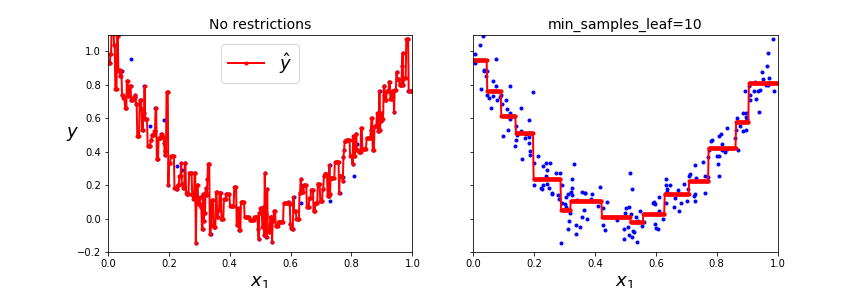
\includegraphics[scale=0.45]{Images/tree_regression_regularization_plot.png}
\end{center}

\subsection{Instability}

Although Decision Trees are a very powerful algorithm, they do have their own limitations. Firstly, Decision Trees tend to use orthogonal
decision boundaries (i.e., splits are perpendicular to an axis), which makes them sensitive to training set rotations. For example, in the 
figure below we can see that the left-hand plot is easily split by a decision tree, however, if we rotate the data 45 degrees, the decision 
boundary looks to be unnecessarily complex. This then causes further issues with the model not being able to generalize well. One thing to fix 
this issue is to use Principal Component Analysis (PCA) which often results in better orientation in the data.

\begin{center}
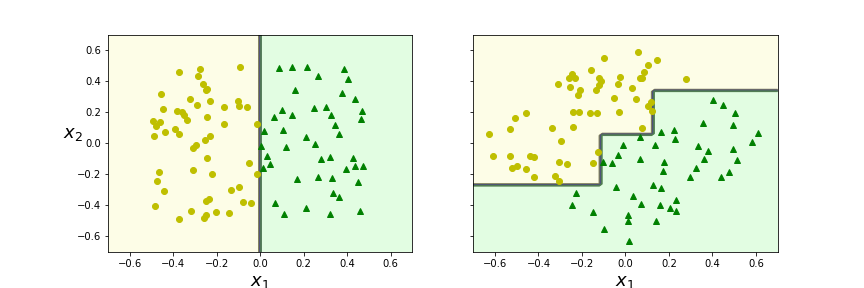
\includegraphics[scale=0.45]{Images/sensitivity_to_rotation_plot.png}
\end{center}

\noindent
However, the main issue with Decision Trees is that they tend to be very sensitive to small variations in the training data. For example, if we 
were to remove the widest \textit{Iris Veriscolor} from the iris training set and train a new Decision Tree, we will get a model that is 
totally different from the model we initially trained. Below will be the plot of the new decision boundaries of the decision tree that does 
not include the widest iris.

\begin{center}
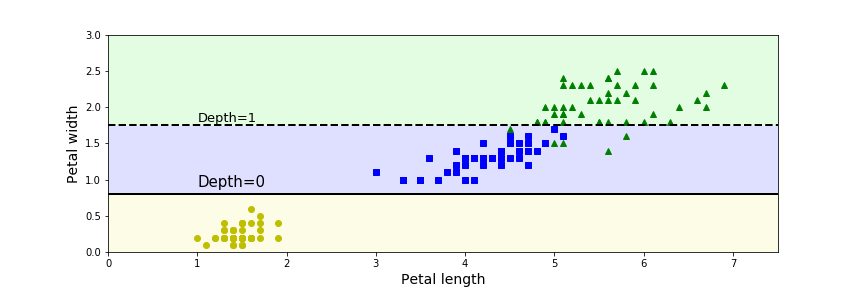
\includegraphics[scale=0.45]{Images/decision_tree_instability_plot.png}
\end{center}

\noindent
As we will see in the next section, Random Forests can limit this instability affect by averaging predictions over many trees.


\section{Random Forest/Ensemble Learning}

\subsection{Decision Trees}

\subsection{Random Forests}

\subsection{Voting Classifiers}

\subsection{Bagging and Pasting}

\subsection{Boosting}

\subsection{Stacking}


\section{Dimensionality Reduction}

Many problems in Machine Learning involve thousands or even millions of features for each training instance.
Having this many features often make training very slow and also make it much harder to find a good solution
as well (Due to the \textit{Curse of Dimensionality}, will be explained more later). \\

\noindent
However, we are often able to reduce the number of features quite considerably, turning a rather complex 
problem into something more simple and/or manageable. Although, we should take care in how we reduce dimensions
as we do lose information with each dimension that we remove. So, if training isn't too slow, we should always
first try to train the system with the original dataset before considering reducing dimensionality. \\

\noindent 
In addition, there are some cases where reducing dimensionality of the training data may filter out some noise
and thus result in higher performance, but in general it will not increase performance and will only decrease
the amount of time it will take to train the model.

\subsection{Curse of Dimensionality}

Given that we are living in 3-dimensional space (4th including time), our understanding of anything above
3-dimensions is incredibly hard to grasp. It also turns out that many things behave very differently in 
high-dimensional space (Please see below). \\

\noindent
\textbf{Expected Distance Between 2 Randomly Chosen Points in Different Dimensions}
\begin{itemize}
    \item \textbf{Unit Square}
        \begin{itemize}
            \item Distance on Average is roughly 0.52
        \end{itemize}
    \item \textbf{Unit 3D Cube}
        \begin{itemize}
            \item Distance on Average is roughly 0.66
        \end{itemize}
    \item \textbf{1 Million Dimensional Hypercube}
        \begin{itemize}
            \item Distance on Average is roughly 408.25 ($\sqrt{\frac{1,000,000}{6}}$)
        \end{itemize}
\end{itemize}

\noindent
Therefore, as a result of above, we can see that high-dimensional datasets are at risk of being very sparse:
most training instances are likely to be far away from each other. This also means that a new instance will
likely be far away from any training instance, making predictions much less reliable compared to a lower 
dimensional model. \\

\noindent
In short, we see that the more dimensions we add, the higher the risk of overfitting the data with our model.

\subsection{Main Approaches for Dimensionality Reduction}

Before taking a look at specific algorithms to reduce dimensionality, it is important to first take a look at
the two main approaches in reducing dimensionality: \textit{Projection} and \textit{Manifold Learning}.

\subsubsection{Projection}

In many cases we will find that the training data we will be using is not spread out uniformly across all
dimensions. Many features will tend to be constant, while others may be highly correlated. Therefore, we find
that many of the training instances lie within (or close to) a much lower-dimensional subspace of the 
high-dimensional space. \\

\noindent
Generally, projection works best when the data we are trying to project to lower dimensions does not have too
many twists and turns that may cause points to overlap each other when brought down to lower dimensions. A
good example to see this will be using the \textit{Swiss Roll} dataset that can be found in Scikit-Learn's
library.

\subsubsection{Manifold Learning}

In the previous section the \textit{Swiss Roll} data set was mentioned, this is an example of a 2D manifold.
In layman's terms, a 2D manifold is a 2D shape that can be bent and twisted in a higher-dimensional space. More
generally, a $d$-dimensional manifold is a part of an $n$-dimensional space where ($d < n$) that locally 
resembles a d-dimensional hyperplane. In the case of the swiss roll, $d = 2$ and $n = 3$: thus, it locally
resembles a 2D plane, but it is rolled in the third dimension. \\

\noindent 
In practice, many dimensionality reduction algorithms work by modeling the manifold on which the training
instances lie; this is called \textit{manifold learning}. The prior relies on the \textit{manifold assumption},
also known as the \textit{manifold hypothesis}, which holds that most real-world high-dimensional datasets lie
close to a much lower-dimensional manifold. Empirically, this assumption is very commonly observed.

\subsection{Principal Compenents Analysis (PCA)}

\textit{Principal Components Analysis} or PCA, for short, is by far one of the most-popular dimensionality
reduction algorithms. In its most basic terms, PCA identifies a hyperplane that lies closest to the data,
and then it projects the data onto it.

\subsubsection*{Principal Components}

When projecting training data onto a lower-dimensional plane, it is important that we are choosing the correct
hyperplane. The algorithm PCA identitifies the axis that accounts for the largest amount of variance in the 
training set (Here variance can be thought of the amount of information captured from a single hyperplane
that the training data is laying on). \\

\noindent
PCA finds as many axes as there are dimensions in the dataset, however, it does this is such a way where it finds
the planes that contain the most amount of variance first and then they decrease in each component (Note, that 
each component is orthogonal to each of the previous axes). \\ 

\noindent
Here we can say that the $i^{th}$ axis is the $i^{th}$ \textit{principal component} (PC) of the data. It is important
to know that for each principal component, PCA finds a zero-centered unit vector pointing in the direction of the PC.
Since two opposing unit vectors lie on the same axis, the direction of the unit vectors returned by PCA are inherently
not stable. For example, if we were to peturb the training data slightly and run PCA on the data, the unit vectors 
may point in the opposite direction as the original vectors in the non perturbed dataset. However, in the grand 
scheme of things, this unstable chracteristic generally does not matter as the unit vectors, regardless of direction, 
tend to lie on the same axes, therefore, the plane will be the same. \\

\noindent
PCA uses a standard matrix decomposition technique called \textit{Singular Value Decomposition} (SVD) that can
decompose the training set matrix $\vec{X}$ into the matrix multiplication of three matrices 
$\vec{U}\vec{\Sigma}\vec{V}^{\intercal}$, where $\vec{V}$ contains the unit vectors that define all the principal
components that we are looking for, as shown below:

$$\vec{V} =
\begin{pmatrix}
| & | &  & | \\
\vec{c_{1}} & \vec{c_{2}} & \cdots & \vec{c_{n}} \\
| & | &  & |
\end{pmatrix}$$

\noindent
Below will be using NumPy's \mintinline{python}{svd()} function to obtain all the principal components of some given
matrix $\vec{X}$:

\begin{minted}{python}
import numpy as np

X_centered = X - X.mean(axis=0) # Centering Matrix
U, s, Vt = np.linalg.svd(X_centered)
c1 = Vt.T[:, 0] # First Principal Component
c2 = Vt.T[:, 1] # Second Principal Component
\end{minted}

\noindent
\textbf{Important}: PCA assumes that the dataset is centered around the origin. However, in Scikit-Learn's PCA classes,
centering is automatically taken care of for you. But if you implement PCA yourself, or if you are using other libraries,
\textbf{do not} forget to center the data first. 

\subsubsection*{Projecting Down to d Dimensions}

Once all principal components of a datset are identified, we can reduce the dimensionality of the dataset down to
\textit{d} dimensions by projecting it onto the hyperplane defined by the first \textit{d} principal components. Selecting
the first few hyperplanes will ensure that the projection we are doing will preserve the most variance as possible. \\

\noindent
To project the training set onto the hyperplane and obtain a reduced $\vec{X}_{d-proj}$ of dimensionality \textit{d},
compute the matrix multiplication of the training set $\vec{X}$ by the matrix $\vec{W}_{d}$, defined as the matrix
the matrix containing the first \textit{d} columns of $\vec{V}$, as shown below:

$$\vec{X}_{d-proj} = \vec{X} \vec{W}_{d}$$

\noindent
The following Python code will be projecting the training set ($\vec{X}$) onto the plane defined by the first two
principal components:

\begin{minted}{python}
W2 = Vt.T[:, :2]
X2D = X_centered.dot(W2)
\end{minted}

\noindent
Thus, that is how we can manually reduce dimensionality of a dataset down to any number of dimensions that we desire to
acquire.

\subsubsection*{Using Scikit-Learn for PCA}

Scikit-Learn's \mintinline{python}{PCA} class uses SVD decomposition to implement PCA (as we have manually done before).
The following code in this section will be covering how to use Scikit-Learns built-in PCA function.\\

\noindent
First we can import PCA in the following way (note that in Scikit-Learn centering is done automatically):

\begin{minted}{python}
from sklearn.decomposition import PCA

pca = PCA(n_components=2) # Only want the first 2 principal components
X2D = pca.fit_transform(X) # Projecting X down to 2 dimensions
\end{minted}

\noindent
Further, after fitting the \mintinline{python}{PCA} transformer to the dataset, the attribute \mintinline{python}{components_}
holds the transpose of $\vec{W}_{d}$ (e.g., the unit vector that defines the first principal component is equal to 
\mintinline{python}{pca.components_.T[:, 0]}) \\

\noindent
A useful variable that is provided by Scikit-Learn's \mintinline{python}{PCA} class is the \mintinline{python}{explained_variance_ratio_}
variable. This variable indicates the proportion of the dataset's variance that lies along each principal component.
We can all the variable in the following way:

\begin{minted}{python}
pca.explained_variance_ratio_

'''
Example output for 2 principal compoenents would be:
array([0.84248607, 0.14631839])
'''
\end{minted}

\noindent
Here that example output is telling us that 84\% of the dataset's variance lies along the first PC, and 14\% lies along
the second PC. This leaves approximately 2\% of the variance to be in the rest of the PCs.

\subsubsection*{Choosing the Right Number of Dimensions}

In practice, we should not be arbitrarily choosing the numbers that we will want to reduce our dataset down to. Luckily,
in Scikit-Learn's PCA class we are able to define the argument \mintinline{python}{n_components} to a number between
0 and 1. For example, if we set the argument, \mintinline{python}{n_components} equal to 0.95, then we will be asking
to return the number of components that preserve 95\% of the data's variance. Below will be an example of implementing
this using Scikit-Learn:

\begin{minted}{python}
pca = PCA(n_components=0.95)
X_reduced = pca.fit_transform(X_train)
# Here X_train is just some random variable that is used for example 
# purposes.
\end{minted}

\noindent
\textbf{Note:} A very good dataset to see the benefits of PCA is applying it to the MNIST dataset (Can be found in Scikit-Learn)
that has about 60,000 images of handwritten notes. One will find that using PCA we can preserve 95\% of the variance in
that dataset even though we reduce the total dimensions down to just over 150 from 784 features (Almost less than 
20\% of the original size of the dataset). 

\subsection{Kernel PCA}

\subsection{Locally Linear Embedding (LLE)}

\subsection{Other Dimensionality Reduction Techniques}


\section{Unsupervised Learning}

\subsection{Clustering}

\subsection{Gaussian Mixtures}

\end{document}